\documentclass[mathserif, handout]{beamer}
% ======================================================================
% General LaTeX Setup for Beamer (Reusable Preamble)
% Author: Chandra Gummaluru
% ======================================================================

\documentclass[mathserif, handout]{beamer}
\setbeamertemplate{frametitle}{}

% ------------------------------------------------------------
% basic packages
% ------------------------------------------------------------
\usepackage{url}
\usepackage{ifthen}
\usepackage{enumerate}
\usepackage[font=small]{caption}
\usepackage{subcaption}
\usepackage{moresize}
\usepackage[outline]{contour}
\usepackage{transparent}
\usepackage{worldflags}
\usepackage{bm}
\usepackage{graphbox}
\usepackage{mathtools}
\usepackage{multirow}
\usepackage{fontawesome5}
\usepackage{pifont}
\usepackage{array}
\usepackage{comment}

% ------------------------------------------------------------
% math
% ------------------------------------------------------------
\DeclarePairedDelimiter{\floor}{\lfloor}{\rfloor}
\DeclarePairedDelimiter{\ceil}{\lceil}{\rceil}

% ------------------------------------------------------------
% colors
% ------------------------------------------------------------
\definecolor{hl}{RGB}{248,196,69}
\definecolor{myred}{HTML}{ED5565}
\definecolor{myorange}{HTML}{FC6E51}
\definecolor{myyellow}{HTML}{FFCE54}
\definecolor{mycyan}{HTML}{4FC1E9}
\definecolor{myblue}{HTML}{5D9CEC}

\newcommand{\graytext}[1]{\footnotesize\color{gray}#1\normalsize\color{black}}

% ------------------------------------------------------------
% symbols
% ------------------------------------------------------------
\newcommand{\cmark}{\ding{51}}
\newcommand{\xmark}{\ding{55}}

% ------------------------------------------------------------
% highlighting
% ------------------------------------------------------------
\newcommand{\reducedstrut}{\vrule width 0pt height .9\ht\strutbox depth .9\dp\strutbox\relax}
\newcommand{\highlight}[1]{%
  \begingroup\setlength{\fboxsep}{0pt}\colorbox{hl}{\reducedstrut$\displaystyle #1$\/}\endgroup}
\newcommand{\highlightc}[2]{%
  \begingroup\setlength{\fboxsep}{0pt}\colorbox{#1}{\reducedstrut$\displaystyle #2$\/}\endgroup}

% ------------------------------------------------------------
% environments (boxes)
% ------------------------------------------------------------
\usepackage{tcolorbox}
\tcbuselibrary{skins}

\newtcolorbox{thmbox}[1][]{colback=gray!30!white!20, colframe=black, fonttitle=\bfseries, title=#1, boxrule=0.5pt}

% 1) Bottom open (draw top + sides only)
\newtcolorbox{thmboxtop}[1][]{
    enhanced,
    frame hidden,
    colback=gray!30!white!20,
    borderline north={0.5pt}{0pt}{black}, % top
    borderline west={0.5pt}{0pt}{black},  % left
    borderline east={0.5pt}{0pt}{black}   % right
}

% 2) Top open (draw bottom + sides only)
\newtcolorbox{thmboxbot}[1][]{
    enhanced,
    frame hidden,
    colback=gray!30!white!20,
    borderline south={0.5pt}{0pt}{black}, % bottom
    borderline west={0.5pt}{0pt}{black},  % left
    borderline east={0.5pt}{0pt}{black}   % right
}

% 3) Side only (draw only left and right)
\newtcolorbox{thmboxside}[1][]{
    enhanced,
    frame hidden,
    colback=gray!30!white!20,
    borderline west={0.5pt}{0pt}{black},  % left
    borderline east={0.5pt}{0pt}{black}   % right
}

\newtcolorbox{defboxtop}[1][]{
    enhanced,
    colback=gray!30!white!20,
    frame hidden,
    overlay={
        % Draw top + sides with rounded corners
        \draw[line width=0.5pt, black, rounded corners=3mm]
            (frame.south west) -- (frame.north west) -- (frame.north east) -- (frame.south east);
    },
    #1
}

\newtcolorbox{defboxbot}[1][]{
    enhanced,
    colback=gray!30!white!20,
    frame hidden,
    overlay={
        % Draw top + sides with rounded corners
        \draw[line width=0.5pt, black, rounded corners=3mm]
            (frame.north west) -- (frame.south west) -- (frame.south east) -- (frame.north east);
    },
    #1
}

\newtcolorbox{defboxside}[1][]{
    enhanced,
    frame hidden,
    colback=gray!30!white!20,
    borderline west={0.5pt}{0pt}{black},  % left
    borderline east={0.5pt}{0pt}{black}   % right
}

\newtcolorbox{proofbox}[1][]{colback=gray!20!white!20, colframe=grey, fonttitle=\bfseries, title=#1, boxrule=0.5pt, colbacktitle=white, enhanced jigsaw, sharp corners}

% ------------------------------------------------------------
% code listings
% ------------------------------------------------------------
\usepackage{listings}
\lstdefinestyle{mypython}{
  language=Python,
  deletekeywords=[2]{open, next, from, chr, str, int},
  morekeywords=[3]{List, Graph, Tree, Dict, Set, UnionFind, Ordict, Trie, Queue},
  morekeywords=[4]{ListNode, Vertex, Edge, Path, TreeNode, DictNode, UnifNode, OrdictNode, TrieNode, QueueNode},
  morekeywords=[5]{True, False, Boolean, String, Integer, Key, Function, KeyedObject, Object, Array, Tuple, Optional, None},
  keywordstyle=\color{mycyan}\bfseries,
  keywordstyle=[3]\color{myblue}\bfseries,
keywordstyle=[4]\color{myblue}\bfseries,
keywordstyle=[5]\color{mycyan}\bfseries,
  stringstyle=\color{orange},
  commentstyle=\color{gray}\itshape,
  basicstyle=\ttfamily\footnotesize,
  numbers=left,
  numberstyle=\tiny\color{gray},
  stepnumber=1,
  numbersep=5pt,
  xleftmargin=15pt,
  frame=none,
  showstringspaces=false,
  breaklines=true,
  breakatwhitespace=true,
  tabsize=4,
  columns=flexible
}


% ------------------------------------------------------------
% algorithms
% ------------------------------------------------------------
\usepackage{algorithm}
\usepackage[endLComment=~]{algpseudocodex}
\makeatletter
\algrenewcommand\ALG@beginalgorithmic{\footnotesize}
\makeatother

% ------------------------------------------------------------
% optimization environments
% ------------------------------------------------------------
\usepackage[nocomma]{optidef}

% ------------------------------------------------------------
% pgfplots and pie charts
% ------------------------------------------------------------
\usepackage{pgfplots}
\usepackage{pgf-pie}
\pgfplotsset{compat=1.7}

% ------------------------------------------------------------
% tikz
% ------------------------------------------------------------
\usepackage{tikz}
\usetikzlibrary{
  angles, quotes, positioning, fit, backgrounds, shapes.geometric, intersections,
  calc, shapes, mindmap, decorations.text, arrows, arrows.meta,
  automata, chains, decorations.pathreplacing, calligraphy,
  decorations.markings, shapes.misc, decorations.pathmorphing
}
\tikzset{
  invisible/.style={opacity=0},
  visible on/.style={alt=#1{}{invisible}},
  alt/.code args={<#1>#2#3}{\alt<#1>{\pgfprioritysalso{#2}}{\pgfprioritysalso{#3}}}
}

\newcommand{\multiedge}[5][]{
\pgfmathsetmacro{\N}{#4}
\pgfmathsetmacro{\mid}{(\N-1)/2}
\foreach \i in {0,...,\numexpr#4-1\relax} {

\pgfmathsetmacro{\k}{\i-\mid}
\draw[#1] ($ (#2) + \k*#5*($(#2)!1!90:(#3)$) $) -- ($ (#3) + \k*#5*($(#2)!1!90:(#3)$) $); 

}
\draw[#1,  -{>[scale=1]}]
  ($(#2)!0.54!(#3)$) -- ($(#2)!0.55!(#3)$);
}

% ------------------------------------------------------------
% bibliography
% ------------------------------------------------------------
\usepackage[style=ieee]{biblatex}
\setbeamertemplate{bibliography item}{\insertbiblabel}
\setbeamertemplate{background canvas}{
  \begin{tikzpicture}[remember picture,overlay]
    \node[opacity=0.0075]
      at (current page.center)
      {
\includegraphics[width=0.8\paperwidth]{images/signature.pdf}};
  \end{tikzpicture}
}

% ------------------------------------------------------------
% beamer theme and settings
% ------------------------------------------------------------
\usetheme{Boadilla}
\usecolortheme{seagull}
\beamertemplatenavigationsymbolsempty
\setbeamertemplate{enumerate item}{(\arabic{enumi})}
\setbeamertemplate{enumerate subitem}{(\alph{enumii})}
\setbeamertemplate{enumerate subsubitem}{(\roman{enumiii})}
\setbeamertemplate{itemize item}[circle]
\setbeamertemplate{itemize subitem}{\circ}
\setbeamertemplate{itemize subsubitem}{-}
\setbeamercolor{item}{fg=black!40}
\setbeamercovered{transparent=10}

% ===========================
% Premade TikZ Figure Commands
% ===========================

% images w/ labels
% inside tikz as a node
\NewDocumentCommand{\labeledimgnodetikz}{O{} m m m m m m}{%
	\begin{scope}[transparency group, #1]
		\node[
			draw,
			circle,
			inner sep=0,
			outer sep=0,
			minimum size=10mm,
			#1
		] (#5) at (#3,#4)
		{\includegraphics[scale=#7]{#6}};
		\node[
			rectangle,
			draw=black,
			thick,
			fill=black!55,
			rounded corners=0.1mm,
			inner sep=0pt,
			outer sep=0pt,
			minimum size=2.8mm,
			minimum width=3.5mm
		] at (#3,#4-0.1) {};
		\node[outer sep=0, inner sep=0, white] at (#3,#4-0.1) {\footnotesize #2};
	\end{scope}
}

% inside tikz isolated

% outside tikz
\NewDocumentCommand{\labelednode}{m}{%
	\begin{tikzpicture}[baseline={(0,-1mm)}]
		\node[
			rectangle,
			thick,
			draw=black,
			fill=black!55,
			rounded corners=0.1mm,
			inner sep=0pt,
			outer sep=0pt,
			minimum size=2.8mm,
			minimum width=3.5mm
		] at (0,0) {};
		\node[outer sep=0, inner sep=0, white, minimum size=2.8mm, minimum width=3.5mm] at (0,0) {\footnotesize #1};
	\end{tikzpicture}
}

% images only
% inside tikz as a node
\NewDocumentCommand{\imgnodetikz}{O{} m m m m m m}{%
	\begin{scope}[transparency group, #1]
		\node[
			draw,
			circle,
			inner sep=0,
			outer sep=0,
			minimum size=10mm,
			#1
		] (#5) at (#3,#4)
		{\includegraphics[scale=#7]{#6}};
		\node[
			rectangle,
			draw,
			thick,
			fill=black!55,
			rounded corners=0.1mm,
			inner sep=0pt,
			outer sep=0pt,
			minimum size=2.8mm,
			minimum width=3.5mm,
			opacity=0
		] at (0,0) {};
		\node[outer sep=0, inner sep=0, white, opacity=0] at (0,0) {\footnotesize #2};
	\end{scope}
}

% inside tikz isolated
\NewDocumentCommand{\imgtikz}{O{} mm}{%
	\begin{scope}[transparency group, #1]
		\node[
			inner sep=0,
			outer sep=0
		] (#5) at (#3,#4)
		{\includegraphics[scale=#3]{#2}};
	\end{scope}
}


% outside tikz
\NewDocumentCommand{\imgnode}{mm}{%
	\begin{tikzpicture}[baseline={(0,-1mm)}]
        \node[
            inner sep=0,
            outer sep=0,
            draw opacity=0,
        ] at (0,0)
        {\includegraphics[scale=#2]{#1}};
    \end{tikzpicture}
}

% outside tikz (inline)
\newcommand{\imgnodetext}[2]{%
	\hspace{-0.5mm}%
	\raisebox{-0.26\height}{%
		\includegraphics[scale=#2]{#1}%
	}%
	\hspace{-0.5mm}%
}


% labels only
% inside tikz as a node
\NewDocumentCommand{\labeltikz}{m}{%
	\node[
		rectangle,
		thick,
		draw=black,
		fill=black!55,
		rounded corners=0.1mm,
		inner sep=0pt,
		outer sep=0pt,
		minimum size=2.8mm,
		minimum width=3.5mm
	] at (0,0) {};
	\node[outer sep=0, inner sep=0, white, draw opacity=0] at (0,0) {\footnotesize #1};
}

% inside tikz isolated

% outside tikz

% === define custom pgfkeys ===
\pgfkeys{
	/devicenode/.is family, /devicenode,
	outline thickness/.initial=thick,
	outline color/.initial=black
}

\NewDocumentCommand{\qpacket}{m}{%
	\begin{tikzpicture}[baseline=(current bounding box.center)]
		\node at (0.5,0.4) {\includegraphics[scale=0.1]{#1}};
	\end{tikzpicture}%
}

\NewDocumentCommand{\bpacketid}{mmm}{%
	\begin{tikzpicture}[baseline=(current bounding box.center)]
		\begin{scope}[shift={(0.85,0.7)}]
			\draw[thick, draw=black, fill=#1, rounded corners=1pt] (0.01,0.05) rectangle node[white, text width=1cm, align=center] {\color{#3}\footnotesize #2} (-0.71,-0.625);
		\end{scope}
	\end{tikzpicture}%
}

\NewDocumentCommand{\packetid}{mmmm}{%
	\begin{tikzpicture}[baseline=(current bounding box.center)]
		\begin{scope}[shift={(0.85,0.7)}]
			\draw[thick, draw=black, fill=#2, rounded corners=1pt] (0.01,0.05) rectangle node[white, text width=1cm, align=center] {\color{#4}\footnotesize #3} (-0.71,-0.625);
			\node[
				star,
				star points=30,
				star point ratio=0,
				scale=1.5,
				draw=black,
				thick,
				fill=white,
				rounded corners=0.1mm,
				inner sep=0pt,
				minimum size=2.8mm
			] at (0,0) {};
			\node at (0,0) {\footnotesize #1};
		\end{scope}
	\end{tikzpicture}%
}

\tikzset{
	dictnode/.pic={
			\draw[thick, fill=#1, line join=]
			(-0.75,-0.5) --
			(-0.75,0.5)  --
			(0.75,0.5) --
			(0.75,-0.5) --
			cycle --
			(-0.75, 0.75) --
			(0.75, 0.75) --
			(0.75, -0.5) --
			cycle;
		}
}

\tikzset{
	queuenode/.pic={
			\draw[thick, fill=#1, line join=round]
			(-0.85,-0.5) --
			(-0.85,0.5)  --
			(0.65,0.5) --
			(0.75,0) --
			(0.65,-0.5) --
			cycle;
		}
}

\tikzset{
	queuenodetail/.pic={
			\draw[thick, fill=#1, line join=round]
			(-0.75,-0.5) --
			(-0.75,0.5)  --
			(0.65,0.5) --
			(0.75,0) --
			(0.65,-0.5) --
			cycle;
		}
}

\tikzset{
	listnode/.style={
			shape=rectangle,
			rounded corners,
			thick,
			minimum height=10mm,
			minimum width=15mm,
			inner sep=0pt
		}
}

\tikzset{
	arraynode/.style={
			shape=rectangle,
			thick,
			minimum height=10mm,
			minimum width=15mm,
			inner sep=0pt
		}
}

\tikzset{
	graphnode/.style={
			shape=circle,
			thick,
			minimum size=5mm,
			inner sep=0pt
		}
}

\tikzset{
	defaultnode/.style={
			transform shape,
			circle,
			draw=black,
			thick,
			fill=white,
			minimum size=10mm,
			inner sep=0pt
		},
	newnode/.style={
			transform shape,
			defaultnode,
			draw=myyellow,
			fill=myyellow!60,
			very thick
		},
	newnodelight/.style={
			transform shape,
			defaultnode,
			draw=myyellow,
			fill=myyellow!30,
			very thick
		},
	deletenode/.style={
			defaultnode,
			draw=gray,
			dashed,
			fill=lightgray,
			text=gray,
			very thick
		},
	nooutlinenode/.style={
			defaultnode,
			draw=none,
            draw opacity=0,
			text=black,
			very thick
		},
    nofillnode/.style={
			defaultnode,
			fill=none,
            text=black,
			very thick
		}
}
\tikzset{
	faded/.style={opacity=0.5, text opacity=0.5, transparency group}
}
\tikzset{
	smallgraytext/.style={font=\footnotesize\color{gray}}
}
\tikzset{
	graytext/.style={font=\normalsize\color{gray}}
}
\tikzset{
  squigglearrow/.style={
    very thick,
    lightgray,
    decorate,
    decoration={
      snake,
      amplitude=1.75pt,
      segment length=8pt
    }
  }
}



% title
\title{Dictionaries}
\subtitle{Algorithms and Data Structures}
\author[C. Gummaluru]{Chandra Gummaluru}
\titlegraphic{
\includegraphics[width=0.15\linewidth]{images/signature.pdf}}
\institute[]{\url{chandra-gummaluru.github.io} }
\date[Algorithms and Data Structures]{}

\begin{document}

\begin{frame}
	\maketitle
\end{frame}

\begin{frame}
	\begin{center}
		\Large \highlight{\textbf{motivation}}
	\end{center}

\end{frame}


\begin{frame}{Motivation}
	When a device (\imgnodetext{images/server.png}{0.0325}) finds the best route to send a message to another device (\imgnodetext{images/phone.png}{0.0325}), it stores this information in a routing table.
	\begin{figure}
		\centering
		\begin{tikzpicture}[scale=0.8, transform shape]
			\labeledimgnodetikz[defaultnode]{\footnotesize\texttt{A}}{1.5}{2}{tA}{images/radio_tower.png}{0.044};
			\labeledimgnodetikz[defaultnode]{\footnotesize\texttt{B}}{3}{0}{tB}{images/radio_tower.png}{0.044};
			\labeledimgnodetikz[defaultnode]{\footnotesize\texttt{C}}{4}{2}{tC}{images/radio_tower.png}{0.044};
			\labeledimgnodetikz[defaultnode]{\footnotesize\texttt{D}}{6}{0.5}{tD}{images/radio_tower.png}{0.044};
			\labeledimgnodetikz[defaultnode]{\footnotesize\texttt{E}}{8}{2}{tE}{images/radio_tower.png}{0.044};

			\imgnodetikz[newnodelight]{empty}{0}{0.5}{server}{images/server.png}{0.052};
			\imgnodetikz[newnode]{empty}{6.5}{3}{phone}{images/phone.png}{0.052};
			\imgnodetikz[defaultnode]{empty}{7.5}{-1}{computer}{images/computer.png}{0.052};
			\imgnodetikz[defaultnode]{empty}{9.5}{0.5}{router}{images/router.png}{0.052};

			\draw[newnode, ->] (server) edge node[midway, above left] {$4$} (tA);
			\draw[defaultnode] (server) edge node[midway, below] {$8$} (tB);

			\draw[defaultnode] (tA) edge node[midway, left] {$11$} (tB);
			\draw[newnode, ->] (tA) edge node[midway, above] {$8$} (tC);

			\draw[defaultnode] (tB) edge node[midway, left] {$7$} (tC);
			\draw[defaultnode] (tB) edge node[midway, below] {$1$} (tD);

			\draw[newnode, ->] (tC) edge node[midway, above] {$2$} (phone);
			\draw[defaultnode] (tC) edge node[midway, above right] {$6$} (tD);

			\draw[defaultnode] (tD) edge node[midway, below left] {$2$} (computer);

			\draw[defaultnode] (phone) edge node[midway, above] {$7$} (tE);
			\draw[defaultnode] (phone) edge node[midway, right] {$4$} (computer);

			\draw[defaultnode] (tE) edge node[midway, right] {$14$} (computer);
			\draw[defaultnode] (tE) edge node[midway, above right] {$9$} (router);

			\draw[defaultnode] (computer) edge node[midway, below right] {$10$} (router);

			\draw[thick, opacity=0.4] (0,0.5) circle (8mm);
			\draw[thick, opacity=0.25] (0,0.5) circle (10.5mm);
			\draw[thick, opacity=0.1] (0,0.5) circle (13mm);
		\end{tikzpicture}
	\end{figure}
	\vspace{-2mm}
	\begin{table}[]
		\centering
		\begin{tabular}{r|c|c|c|c|c|c|c|c}
			\textbf{Target} & \labelednode{\texttt{A}} &
			\labelednode{\texttt{B}} &
			\labelednode{\texttt{C}} &
			\labelednode{\texttt{D}} &
			\labelednode{\texttt{E}} &
			\imgnode{images/phone.png}{0.04} &
			\imgnode{images/computer.png}{0.04} &
			\imgnode{images/router.png}{0.04}\\\hline

			\textbf{Hop}    & \labelednode{\texttt{A}} &
			? &
			\labelednode{\texttt{A}} &
			? &
			? &
			\labelednode{\texttt{A}} &
			? &
			?\\
		\end{tabular}
	\end{table}
	\vspace{-4mm}
	\begin{center}
		\graytext{\imgnode{images/server.png}{0.0325}'s routing table}
	\end{center}
	This allows the device (\imgnodetext{images/server.png}{0.0325}) from having to re-compute the best route.
\end{frame}


\begin{frame}
	\begin{thmbox}
		\begin{center}
			\scalebox{0.75}{\raisebox{-0.3\height}{
\includegraphics[scale=0.05]{images/bulb.png}}}
		\end{center}
		We need a data structure that can quickly retrieve a value at a given key, so we do not have to search through all elements.
	\end{thmbox}
\end{frame}


\begin{frame}{Dictionaries}
	\begin{center}
		\Large \highlight{\textbf{dictionaries}} \\[1mm]
		\normalsize\color{gray} stores items by key \\[3mm]
	\end{center}

	\begin{figure}
		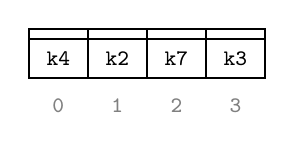
\begin{tikzpicture}

			\tikzset{
				basicnode/.style={
						shape=rectangle,
						draw=black,
						thick,
						fill=white,
						minimum width=10mm,
						minimum height=6mm,
						inner sep=0pt
					}
			}
			\coordinate (m1) at (-2.25,0);
			\coordinate (m2) at (-1.5,0);
			\coordinate (m3) at (-0.75,0);
			\coordinate (m4) at (0,0);

			\begin{scope}[scale=0.5, transform shape]
				\pic at (m4) {dictnode={white}};
				\pic at (m3) {dictnode={white}};
				\pic at (m2) {dictnode={white}};
				\pic at (m1) {dictnode={white}};
			\end{scope}

			\node at (m1) {\footnotesize\texttt{k4}};
			\node at (m2) {\footnotesize\texttt{k2}};
			\node at (m3) {\footnotesize\texttt{k7}};
			\node at (m4) {\footnotesize\texttt{k3}};

			\node[draw=white, text=black] (l1) at (-2.25,-0.6) {\footnotesize\graytext{\texttt{0}}};
			\node[draw=white, text=black] (l2) at (-1.5,-0.6) {\footnotesize\graytext{\texttt{1}}};
			\node[draw=white, text=black] (l3) at (-0.75,-0.6) {\footnotesize\graytext{\texttt{2}}};
			\node[draw=white, text=black] (l4) at (0,-0.6) {\footnotesize\graytext{\texttt{3}}};

		\end{tikzpicture}
	\end{figure}
\end{frame}

\begin{frame}[fragile]
	A \texttt{Dict} stores \texttt{DictNode} objects and supports the following operations:\\~\\
	\begin{itemize}

		\item \highlight{\texttt{get}} \\
		      \graytext{returns an object (if it exists)}\\[-1mm]
		      \begin{lstlisting}[style=mypython]
get(key: Key) -> Optional[DictNode]
\end{lstlisting}

		\item \highlight{\texttt{insert}} \\
		      \graytext{inserts/updates an object}\\[-1mm]
		      \begin{lstlisting}[style=mypython]
insert(key: Key, obj: Object) -> Optional[DictNode]
\end{lstlisting}

		\item \highlight{\texttt{delete}} \\
		      \graytext{removes an object (if it exists)}\\[-1mm]
		      \begin{lstlisting}[style=mypython]
delete(key: Key) -> Optional[DictNode]
\end{lstlisting}

	\end{itemize}
\end{frame}

\begin{frame}[fragile]
	\begin{itemize}

		\item \highlight{\texttt{get\_keys}} \\
		      \graytext{returns an list of keys}\\[-1mm]
		      \begin{lstlisting}[style=mypython]
get_keys() -> List[Key]
\end{lstlisting}

		\item \highlight{\texttt{get\_objs}} \\
		      \graytext{returns a list of objects}\\[-1mm]
		      \begin{lstlisting}[style=mypython]
get_objs() -> List[Object]
\end{lstlisting}

	\end{itemize}
\end{frame}


\begin{frame}{Dictionaries (via Hash Tables)}
	\begin{center}
		\Large \highlight{\texttt{Dict}} \\[1mm] \normalsize \color{gray} (via Hash Tables)
	\end{center}
\end{frame}


\begin{frame}
	We can define a mapping between keys and integers:

	\begin{thmbox}
		A \highlight{\textbf{hash function}} is a function, \( h: \mathcal{U} \rightarrow \mathbb{N} \), that maps keys from a large universe \(\mathcal{U}\) to integers within a fixed range.
	\end{thmbox}
	\begin{figure}
		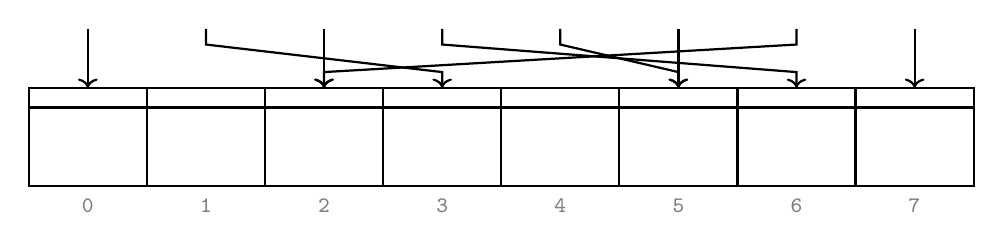
\begin{tikzpicture}

			\begin{scope}
				\begin{scope}[shift={{(-1.5,2)}}]
					\labeltikz{\texttt{A}}
				\end{scope}
				\begin{scope}[shift={{(0,2)}}]
					\labeltikz{\texttt{B}}
				\end{scope}
				\begin{scope}[shift={{(1.5,2)}}]
					\labeltikz{\texttt{C}}
				\end{scope}
				\begin{scope}[shift={{(3,2)}}]
					\labeltikz{\texttt{D}}
				\end{scope}
				\begin{scope}[shift={{(4.5,2)}}]
					\labeltikz{\texttt{E}}
				\end{scope}
				\begin{scope}[shift={{(6,2)}}]
					\imgtikz{images/phone.png}{0.04};
				\end{scope}
				\begin{scope}[shift={{(7.5,2)}}]
					\imgtikz{images/router.png}{0.04};
				\end{scope}
				\begin{scope}[shift={{(9,2)}}]
					\imgtikz{images/computer.png}{0.04};
				\end{scope}
			\end{scope}

			\begin{scope}
				\tikzset{
					downhead/.style={
							thick,
							postaction={decorate,decoration={markings,mark=at position 1 with {\arrow{>}}}}
						}
				}

				\draw[downhead] (-1.5,1.5) -- ++(0,-0.2) -- (-1.5,0.95) -- ++(0,-0.2);
				\draw[downhead] (0,1.5) -- ++(0,-0.2) -- (3,0.95) -- ++(0,-0.2);
				\draw[downhead] (1.5,1.5) -- ++(0,-0.2) -- (1.5,0.95) -- ++(0,-0.2);
				\draw[downhead] (3,1.5) -- ++(0,-0.2) -- (7.5,0.95) -- ++(0,-0.2);
				\draw[downhead] (4.5,1.5) -- ++(0,-0.2) -- (6,0.95) -- ++(0,-0.2);
				\draw[downhead] (6,1.5) -- ++(0,-0.2) -- (6,0.95) -- ++(0,-0.2);
				\draw[downhead] (7.5,1.5) -- ++(0,-0.2) -- (1.5,0.95) -- ++(0,-0.2);
				\draw[downhead] (9,1.5) -- ++(0,-0.2) -- (9,0.95) -- ++(0,-0.2);

			\end{scope}

			\begin{scope}


				\coordinate (mA) at (-1.5,0);
				\coordinate (mB) at (0,0);
				\coordinate (mC) at (1.5,0);
				\coordinate (mD) at (3,0);
				\coordinate (mE) at (4.5,0);
				\coordinate (mF) at (6,0);
				\coordinate (mG) at (7.5,0);
				\coordinate (mH) at (9,0);

				\pic at (mA) {dictnode={white}};
				\pic at (mB) {dictnode={white}};
				\pic at (mC) {dictnode={white}};
				\pic at (mD) {dictnode={white}};
				\pic at (mE) {dictnode={white}};
				\pic at (mF) {dictnode={white}};
				\pic at (mG) {dictnode={white}};
				\pic at (mH) {dictnode={white}};

				\node[smallgraytext] (l1) at (-1.5,-0.75) {\texttt{0}};
				\node[smallgraytext] (l2) at (0,-0.75) {\texttt{1}};
				\node[smallgraytext] (l3) at (1.5,-0.75) {\texttt{2}};
				\node[smallgraytext] (l4) at (3,-0.75) {\texttt{3}};
				\node[smallgraytext] (l5) at (4.5, -0.75) {\texttt{4}};
				\node[smallgraytext] (l6) at (6,-0.75) {\texttt{5}};
				\node[smallgraytext] (l7) at (7.5,-0.75) {\texttt{6}};
				\node[smallgraytext] (l8) at (9,-0.75) {\texttt{7}};


			\end{scope}

		\end{tikzpicture}
	\end{figure}
	\begin{center}
		\graytext{a mapping between keys (devices) and integers}
	\end{center}
\end{frame}



\begin{frame}[fragile]
	\begin{thmboxtop}
		\highlight{\texttt{Dict}} \\
		\graytext{(via Hash Tables)}
		\begin{lstlisting}[style=mypython]
class DictNode:
# attributes
    # the key of this node
    key: Key

    # the object of this node
    obj: Object
\end{lstlisting}
	\end{thmboxtop}
\end{frame}

\begin{frame}[fragile]
	\begin{thmboxbot}
		\begin{lstlisting}[style=mypython]
class Dict:
# attributes
    # an array of lists of nodes
    buckets: Array[List[DictNode]]

    # a hash function
    hash_fnc: Function[[Key], [Integer]]

    # a probe function (used in probing)
    probe_fnc: Function[[Integer], [Integer]]
    
    # the number of nodes in the array (excluding chaining)
    size: Integer

    # the number of spots in the array
    capacity: Integer

# functions
    ...
\end{lstlisting}
	\end{thmboxbot}
\end{frame}

\begin{frame}[fragile]
	\begin{proofbox}
		\begin{lstlisting}[style=mypython]
def get_keys(self: Dict) -> List[Key]
    keys = List[Key]()
    for idx in 0, ..., self.buckets.size - 1:
        keys.append(self.buckets[idx].get(0).key)
    return keys
\end{lstlisting}
	\end{proofbox}
\end{frame}

\begin{frame}[fragile]
	\begin{proofbox}
		\begin{lstlisting}[style=mypython]
def get_nodes(self: Dict) -> List[DictNode]
    nodes = List[DictNode]()
    for idx in 0, ..., self.buckets.size - 1:
        nodes.append(self.buckets[idx].get(0))
    return nodes
\end{lstlisting}
	\end{proofbox}
\end{frame}

\begin{frame}[fragile]
	\begin{proofbox}
		\begin{lstlisting}[style=mypython]
def _hash_fnc(self: Dict, key: Key):
    return self.hash_fnc(key) % self.capacity
\end{lstlisting}
	\end{proofbox}
\end{frame}

\begin{frame}[fragile]
	\begin{proofbox}
		\begin{lstlisting}[style=mypython]
def _resize(self: Dict):
        old_buckets = self.buckets
        old_capacity = self.buckets.size
        self.buckets = Array(2 * self.capacity)
        self.size = 0
        self.capacity *= 2
        for idx = 1, ..., old_capacity:
            if self.old_buckets[idx] is not None:
                key = self.old_buckets[idx].get(0).key
                obj = self.old_buckets[idx].get(0).obj
                self.insert(key, obj)
\end{lstlisting}
	\end{proofbox}
\end{frame}

\begin{frame}
	\begin{center}
		\highlight{\textbf{get}} \\[1mm]
		\footnotesize\color{gray} \texttt{get(k7)}
	\end{center}

	\begin{figure}
		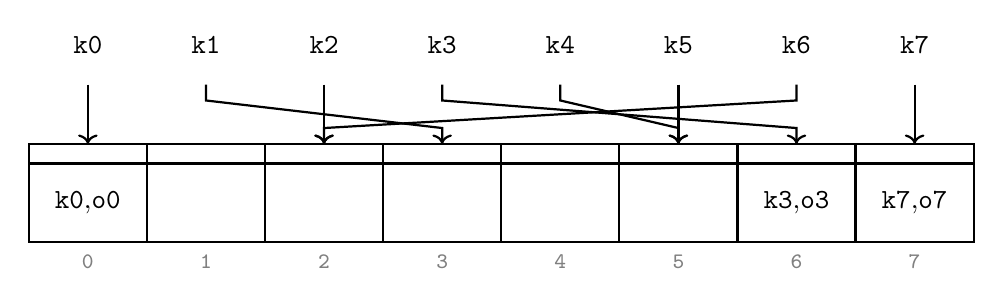
\begin{tikzpicture}

			\begin{scope}
				\begin{scope}[shift={{(-1.5,2)}}]
					\node at (0,0) {\texttt{k0}};
				\end{scope}
				\begin{scope}[shift={{(0,2)}}]
					\node at (0,0) {\texttt{k1}};
				\end{scope}
				\begin{scope}[shift={{(1.5,2)}}]
					\node at (0,0) {\texttt{k2}};
				\end{scope}
				\begin{scope}[shift={{(3,2)}}]
					\node at (0,0) {\texttt{k3}};
				\end{scope}
				\begin{scope}[shift={{(4.5,2)}}]
					\node at (0,0) {\texttt{k4}};
				\end{scope}
				\begin{scope}[shift={{(6,2)}}]
					\node at (0,0) {\texttt{k5}};
				\end{scope}
				\begin{scope}[shift={{(7.5,2)}}]
					\node at (0,0) {\texttt{k6}};
				\end{scope}
				\begin{scope}[shift={{(9,2)}}]
					\node at (0,0) {\texttt{k7}};
				\end{scope}
			\end{scope}

			\begin{scope}
				\tikzset{
					downhead/.style={
							thick,
							postaction={decorate,decoration={markings,mark=at position 1 with {\arrow{>}}}}
						}
				}

				\draw[downhead] (-1.5,1.5) -- ++(0,-0.2) -- (-1.5,0.95) -- ++(0,-0.2);
				\draw[downhead] (0,1.5) -- ++(0,-0.2) -- (3,0.95) -- ++(0,-0.2);
				\draw[downhead] (1.5,1.5) -- ++(0,-0.2) -- (1.5,0.95) -- ++(0,-0.2);
				\draw[downhead] (3,1.5) -- ++(0,-0.2) -- (7.5,0.95) -- ++(0,-0.2);
				\draw[downhead] (4.5,1.5) -- ++(0,-0.2) -- (6,0.95) -- ++(0,-0.2);
				\draw[downhead] (6,1.5) -- ++(0,-0.2) -- (6,0.95) -- ++(0,-0.2);
				\draw[downhead] (7.5,1.5) -- ++(0,-0.2) -- (1.5,0.95) -- ++(0,-0.2);
				\draw[downhead] (9,1.5) -- ++(0,-0.2) -- (9,0.95) -- ++(0,-0.2);

			\end{scope}

			\begin{scope}

				\coordinate (mA) at (-1.5,0);
				\coordinate (mB) at (0,0);
				\coordinate (mC) at (1.5,0);
				\coordinate (mD) at (3,0);
				\coordinate (mE) at (4.5,0);
				\coordinate (mF) at (6,0);
				\coordinate (mG) at (7.5,0);
				\coordinate (mH) at (9,0);

				\pic at (mA) {dictnode={white}};
				\pic at (mB) {dictnode={white}};
				\pic at (mC) {dictnode={white}};
				\pic at (mD) {dictnode={white}};
				\pic at (mE) {dictnode={white}};
				\pic at (mF) {dictnode={white}};
				\pic at (mG) {dictnode={white}};
				\pic at (mH) {dictnode={white}};

				\node[smallgraytext] (l1) at (-1.5,-0.75) {\texttt{0}};
				\node[smallgraytext] (l2) at (0,-0.75) {\texttt{1}};
				\node[smallgraytext] (l3) at (1.5,-0.75) {\texttt{2}};
				\node[smallgraytext] (l4) at (3,-0.75) {\texttt{3}};
				\node[smallgraytext] (l5) at (4.5, -0.75) {\texttt{4}};
				\node[smallgraytext] (l6) at (6,-0.75) {\texttt{5}};
				\node[smallgraytext] (l7) at (7.5,-0.75) {\texttt{6}};
				\node[smallgraytext] (l8) at (9,-0.75) {\texttt{7}};

			\end{scope}

			\node at (mA) {\texttt{k0},\texttt{o0}};
			\node at (mG) {\texttt{k3},\texttt{o3}};
			\node at (mH) {\texttt{k7},\texttt{o7}};

		\end{tikzpicture}
	\end{figure}

	\begin{center}
		\footnotesize\color{gray} compute the hash value of the key
	\end{center}
\end{frame}


\begin{frame}
	\begin{center}
		\highlight{\textbf{get}} \\[1mm]
		\footnotesize\color{gray} \texttt{get(k7)}
	\end{center}

	\begin{figure}
		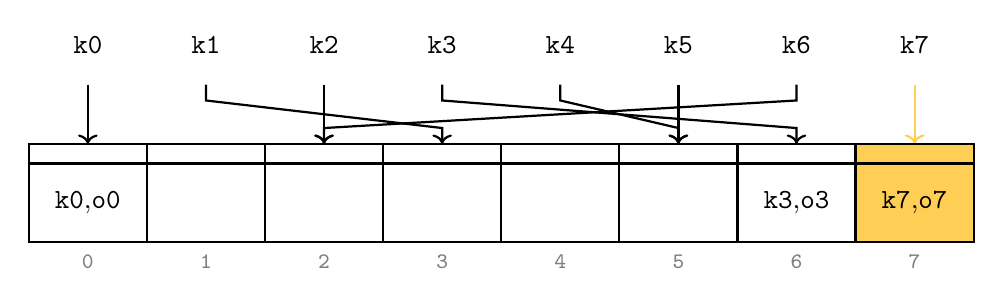
\begin{tikzpicture}

			\begin{scope}
				\begin{scope}[shift={{(-1.5,2)}}]
					\node at (0,0) {\texttt{k0}};
				\end{scope}
				\begin{scope}[shift={{(0,2)}}]
					\node at (0,0) {\texttt{k1}};
				\end{scope}
				\begin{scope}[shift={{(1.5,2)}}]
					\node at (0,0) {\texttt{k2}};
				\end{scope}
				\begin{scope}[shift={{(3,2)}}]
					\node at (0,0) {\texttt{k3}};
				\end{scope}
				\begin{scope}[shift={{(4.5,2)}}]
					\node at (0,0) {\texttt{k4}};
				\end{scope}
				\begin{scope}[shift={{(6,2)}}]
					\node at (0,0) {\texttt{k5}};
				\end{scope}
				\begin{scope}[shift={{(7.5,2)}}]
					\node at (0,0) {\texttt{k6}};
				\end{scope}
				\begin{scope}[shift={{(9,2)}}]
					\node at (0,0) {\texttt{k7}};
				\end{scope}
			\end{scope}

			\begin{scope}
				\tikzset{
					downhead/.style={
							thick,
							postaction={decorate,decoration={markings,mark=at position 1 with {\arrow{>}}}}
						}
				}

				\draw[downhead] (-1.5,1.5) -- ++(0,-0.2) -- (-1.5,0.95) -- ++(0,-0.2);
				\draw[downhead] (0,1.5) -- ++(0,-0.2) -- (3,0.95) -- ++(0,-0.2);
				\draw[downhead] (1.5,1.5) -- ++(0,-0.2) -- (1.5,0.95) -- ++(0,-0.2);
				\draw[downhead] (3,1.5) -- ++(0,-0.2) -- (7.5,0.95) -- ++(0,-0.2);
				\draw[downhead] (4.5,1.5) -- ++(0,-0.2) -- (6,0.95) -- ++(0,-0.2);
				\draw[downhead] (6,1.5) -- ++(0,-0.2) -- (6,0.95) -- ++(0,-0.2);
				\draw[downhead] (7.5,1.5) -- ++(0,-0.2) -- (1.5,0.95) -- ++(0,-0.2);
				\draw[downhead, myyellow] (9,1.5) -- ++(0,-0.2) -- (9,0.95) -- ++(0,-0.2);

			\end{scope}

			\begin{scope}


				\coordinate (mA) at (-1.5,0);
				\coordinate (mB) at (0,0);
				\coordinate (mC) at (1.5,0);
				\coordinate (mD) at (3,0);
				\coordinate (mE) at (4.5,0);
				\coordinate (mF) at (6,0);
				\coordinate (mG) at (7.5,0);
				\coordinate (mH) at (9,0);

				\pic at (mA) {dictnode={white}};
				\pic at (mB) {dictnode={white}};
				\pic at (mC) {dictnode={white}};
				\pic at (mD) {dictnode={white}};
				\pic at (mE) {dictnode={white}};
				\pic at (mF) {dictnode={white}};
				\pic at (mG) {dictnode={white}};
				\pic at (mH) {dictnode={myyellow}};

				\node[smallgraytext] (l1) at (-1.5,-0.75) {\texttt{0}};
				\node[smallgraytext] (l2) at (0,-0.75) {\texttt{1}};
				\node[smallgraytext] (l3) at (1.5,-0.75) {\texttt{2}};
				\node[smallgraytext] (l4) at (3,-0.75) {\texttt{3}};
				\node[smallgraytext] (l5) at (4.5, -0.75) {\texttt{4}};
				\node[smallgraytext] (l6) at (6,-0.75) {\texttt{5}};
				\node[smallgraytext] (l7) at (7.5,-0.75) {\texttt{6}};
				\node[smallgraytext] (l8) at (9,-0.75) {\texttt{7}};

			\end{scope}

			\node at (mA) {\texttt{k0},\texttt{o0}};
			\node at (mG) {\texttt{k3},\texttt{o3}};
			\node at (mH) {\texttt{k7},\texttt{o7}};

		\end{tikzpicture}
	\end{figure}

	\begin{center}
		\footnotesize\color{gray} return node at the index specified by the hash value
	\end{center}
\end{frame}

\begin{frame}[fragile]
	\begin{proofbox}
		\begin{lstlisting}[style=mypython]
def get(self: Dict, key: Key) -> Optional[DictNode]:
    idx = self._hash_fnc(key)
    node = self.buckets[idx].get(0)
    if node is None or node.key is not key:
        return None
    return node
\end{lstlisting}
	\end{proofbox}
\end{frame}



\begin{frame}
	\begin{center}
		\highlight{\textbf{insert}} \\[1mm]
		\footnotesize\color{gray} \texttt{insert(k5,o5)}
	\end{center}


	\begin{figure}
		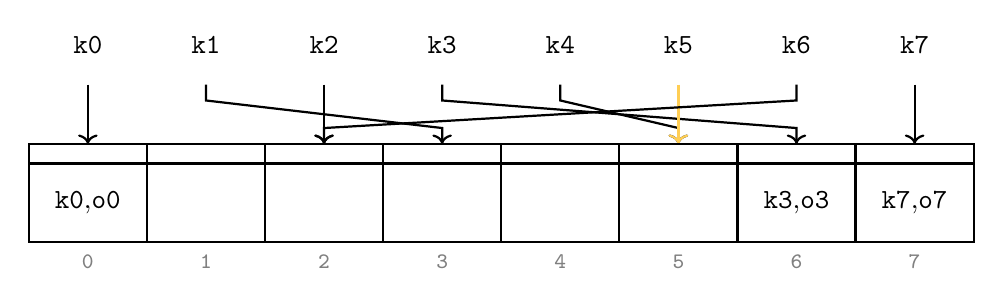
\begin{tikzpicture}

			\begin{scope}
				\begin{scope}[shift={{(-1.5,2)}}]
					\node at (0,0) {\texttt{k0}};
				\end{scope}
				\begin{scope}[shift={{(0,2)}}]
					\node at (0,0) {\texttt{k1}};
				\end{scope}
				\begin{scope}[shift={{(1.5,2)}}]
					\node at (0,0) {\texttt{k2}};
				\end{scope}
				\begin{scope}[shift={{(3,2)}}]
					\node at (0,0) {\texttt{k3}};
				\end{scope}
				\begin{scope}[shift={{(4.5,2)}}]
					\node at (0,0) {\texttt{k4}};
				\end{scope}
				\begin{scope}[shift={{(6,2)}}]
					\node at (0,0) {\texttt{k5}};
				\end{scope}
				\begin{scope}[shift={{(7.5,2)}}]
					\node at (0,0) {\texttt{k6}};
				\end{scope}
				\begin{scope}[shift={{(9,2)}}]
					\node at (0,0) {\texttt{k7}};
				\end{scope}
			\end{scope}

			\begin{scope}
				\tikzset{
					downhead/.style={
							thick,
							postaction={decorate,decoration={markings,mark=at position 1 with {\arrow{>}}}}
						}
				}

				\draw[downhead] (-1.5,1.5) -- ++(0,-0.2) -- (-1.5,0.95) -- ++(0,-0.2);
				\draw[downhead] (0,1.5) -- ++(0,-0.2) -- (3,0.95) -- ++(0,-0.2);
				\draw[downhead] (1.5,1.5) -- ++(0,-0.2) -- (1.5,0.95) -- ++(0,-0.2);
				\draw[downhead] (3,1.5) -- ++(0,-0.2) -- (7.5,0.95) -- ++(0,-0.2);
				\draw[downhead] (4.5,1.5) -- ++(0,-0.2) -- (6,0.95) -- ++(0,-0.2);
				\draw[downhead, myyellow] (6,1.5) -- ++(0,-0.2) -- (6,0.95) -- ++(0,-0.2);
				\draw[downhead] (7.5,1.5) -- ++(0,-0.2) -- (1.5,0.95) -- ++(0,-0.2);
				\draw[downhead] (9,1.5) -- ++(0,-0.2) -- (9,0.95) -- ++(0,-0.2);

			\end{scope}

			\begin{scope}


				\coordinate (mA) at (-1.5,0);
				\coordinate (mB) at (0,0);
				\coordinate (mC) at (1.5,0);
				\coordinate (mD) at (3,0);
				\coordinate (mE) at (4.5,0);
				\coordinate (mF) at (6,0);
				\coordinate (mG) at (7.5,0);
				\coordinate (mH) at (9,0);

				\pic at (mA) {dictnode={white}};
				\pic at (mB) {dictnode={white}};
				\pic at (mC) {dictnode={white}};
				\pic at (mD) {dictnode={white}};
				\pic at (mE) {dictnode={white}};
				\pic at (mF) {dictnode={white}};
				\pic at (mG) {dictnode={white}};
				\pic at (mH) {dictnode={white}};

				\node[smallgraytext] (l1) at (-1.5,-0.75) {\texttt{0}};
				\node[smallgraytext] (l2) at (0,-0.75) {\texttt{1}};
				\node[smallgraytext] (l3) at (1.5,-0.75) {\texttt{2}};
				\node[smallgraytext] (l4) at (3,-0.75) {\texttt{3}};
				\node[smallgraytext] (l5) at (4.5, -0.75) {\texttt{4}};
				\node[smallgraytext] (l6) at (6,-0.75) {\texttt{5}};
				\node[smallgraytext] (l7) at (7.5,-0.75) {\texttt{6}};
				\node[smallgraytext] (l8) at (9,-0.75) {\texttt{7}};

			\end{scope}

			\node at (mA) {\texttt{k0},\texttt{o0}};
			\node at (mG) {\texttt{k3},\texttt{o3}};
			\node at (mH) {\texttt{k7},\texttt{o7}};

		\end{tikzpicture}
	\end{figure}

	\begin{center}
		\footnotesize\color{gray} compute the hash value of the key
	\end{center}
\end{frame}

\begin{frame}
	\begin{center}
		\highlight{\textbf{insert}} \\[1mm]
		\footnotesize\color{gray} \texttt{insert(k5,o5)}
	\end{center}


	\begin{figure}
		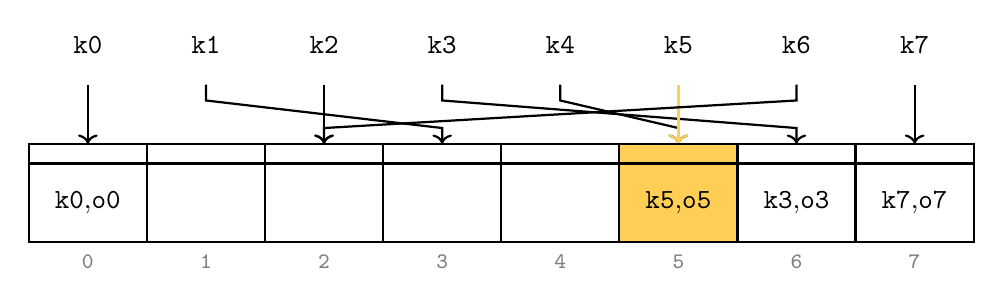
\begin{tikzpicture}

			\begin{scope}
				\begin{scope}[shift={{(-1.5,2)}}]
					\node at (0,0) {\texttt{k0}};
				\end{scope}
				\begin{scope}[shift={{(0,2)}}]
					\node at (0,0) {\texttt{k1}};
				\end{scope}
				\begin{scope}[shift={{(1.5,2)}}]
					\node at (0,0) {\texttt{k2}};
				\end{scope}
				\begin{scope}[shift={{(3,2)}}]
					\node at (0,0) {\texttt{k3}};
				\end{scope}
				\begin{scope}[shift={{(4.5,2)}}]
					\node at (0,0) {\texttt{k4}};
				\end{scope}
				\begin{scope}[shift={{(6,2)}}]
					\node at (0,0) {\texttt{k5}};
				\end{scope}
				\begin{scope}[shift={{(7.5,2)}}]
					\node at (0,0) {\texttt{k6}};
				\end{scope}
				\begin{scope}[shift={{(9,2)}}]
					\node at (0,0) {\texttt{k7}};
				\end{scope}
			\end{scope}

			\begin{scope}
				\tikzset{
					downhead/.style={
							thick,
							postaction={decorate,decoration={markings,mark=at position 1 with {\arrow{>}}}}
						}
				}

				\draw[downhead] (-1.5,1.5) -- ++(0,-0.2) -- (-1.5,0.95) -- ++(0,-0.2);
				\draw[downhead] (0,1.5) -- ++(0,-0.2) -- (3,0.95) -- ++(0,-0.2);
				\draw[downhead] (1.5,1.5) -- ++(0,-0.2) -- (1.5,0.95) -- ++(0,-0.2);
				\draw[downhead] (3,1.5) -- ++(0,-0.2) -- (7.5,0.95) -- ++(0,-0.2);
				\draw[downhead] (4.5,1.5) -- ++(0,-0.2) -- (6,0.95) -- ++(0,-0.2);
				\draw[downhead, myyellow] (6,1.5) -- ++(0,-0.2) -- (6,0.95) -- ++(0,-0.2);
				\draw[downhead] (7.5,1.5) -- ++(0,-0.2) -- (1.5,0.95) -- ++(0,-0.2);
				\draw[downhead] (9,1.5) -- ++(0,-0.2) -- (9,0.95) -- ++(0,-0.2);

			\end{scope}

			\begin{scope}


				\coordinate (mA) at (-1.5,0);
				\coordinate (mB) at (0,0);
				\coordinate (mC) at (1.5,0);
				\coordinate (mD) at (3,0);
				\coordinate (mE) at (4.5,0);
				\coordinate (mF) at (6,0);
				\coordinate (mG) at (7.5,0);
				\coordinate (mH) at (9,0);

				\pic at (mA) {dictnode={white}};
				\pic at (mB) {dictnode={white}};
				\pic at (mC) {dictnode={white}};
				\pic at (mD) {dictnode={white}};
				\pic at (mE) {dictnode={white}};
				\pic at (mF) {dictnode={myyellow}};
				\pic at (mG) {dictnode={white}};
				\pic at (mH) {dictnode={white}};

				\node[smallgraytext] (l1) at (-1.5,-0.75) {\texttt{0}};
				\node[smallgraytext] (l2) at (0,-0.75) {\texttt{1}};
				\node[smallgraytext] (l3) at (1.5,-0.75) {\texttt{2}};
				\node[smallgraytext] (l4) at (3,-0.75) {\texttt{3}};
				\node[smallgraytext] (l5) at (4.5, -0.75) {\texttt{4}};
				\node[smallgraytext] (l6) at (6,-0.75) {\texttt{5}};
				\node[smallgraytext] (l7) at (7.5,-0.75) {\texttt{6}};
				\node[smallgraytext] (l8) at (9,-0.75) {\texttt{7}};

			\end{scope}

			\node at (mA) {\texttt{k0},\texttt{o0}};
			\node at (mG) {\texttt{k3},\texttt{o3}};
			\node at (mH) {\texttt{k7},\texttt{o7}};
			\node at (mF) {\texttt{k5},\texttt{o5}};

		\end{tikzpicture}
	\end{figure}

	\begin{center}
		\footnotesize\color{gray} insert into the index specified by the hash value
	\end{center}
\end{frame}

\begin{frame}[fragile]
	\begin{proofbox}
		\begin{lstlisting}[style=mypython]
def insert(self: Dict, key: Key, obj: Object) -> Optional[DictNode]:
    if self.size is self.capacity:
        self._resize()
    idx = self._hash_fnc(key)
    self.buckets[idx] = DictNode(key, obj)
    self.size += 1
    return self.buckets[idx].get(0)
\end{lstlisting}
	\end{proofbox}
\end{frame}

\begin{frame}
	\begin{center}
		\highlight{\textbf{delete}} \\[1mm]
		\footnotesize\color{gray} \texttt{delete(k5)}
	\end{center}

	\begin{figure}
		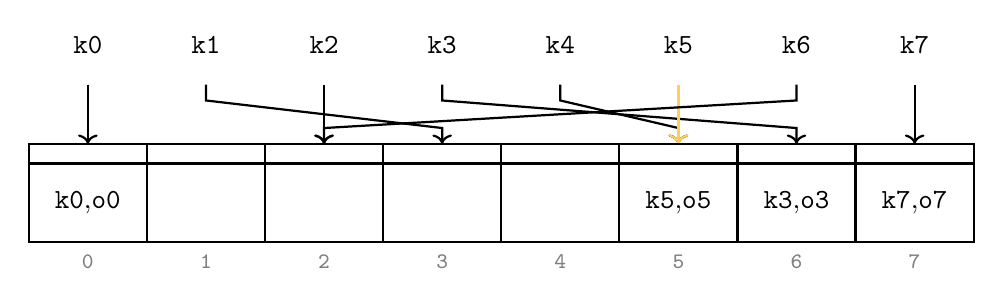
\begin{tikzpicture}

			\begin{scope}
				\begin{scope}[shift={{(-1.5,2)}}]
					\node at (0,0) {\texttt{k0}};
				\end{scope}
				\begin{scope}[shift={{(0,2)}}]
					\node at (0,0) {\texttt{k1}};
				\end{scope}
				\begin{scope}[shift={{(1.5,2)}}]
					\node at (0,0) {\texttt{k2}};
				\end{scope}
				\begin{scope}[shift={{(3,2)}}]
					\node at (0,0) {\texttt{k3}};
				\end{scope}
				\begin{scope}[shift={{(4.5,2)}}]
					\node at (0,0) {\texttt{k4}};
				\end{scope}
				\begin{scope}[shift={{(6,2)}}]
					\node at (0,0) {\texttt{k5}};
				\end{scope}
				\begin{scope}[shift={{(7.5,2)}}]
					\node at (0,0) {\texttt{k6}};
				\end{scope}
				\begin{scope}[shift={{(9,2)}}]
					\node at (0,0) {\texttt{k7}};
				\end{scope}
			\end{scope}

			\begin{scope}
				\tikzset{
					downhead/.style={
							thick,
							postaction={decorate,decoration={markings,mark=at position 1 with {\arrow{>}}}}
						}
				}

				\draw[downhead] (-1.5,1.5) -- ++(0,-0.2) -- (-1.5,0.95) -- ++(0,-0.2);
				\draw[downhead] (0,1.5) -- ++(0,-0.2) -- (3,0.95) -- ++(0,-0.2);
				\draw[downhead] (1.5,1.5) -- ++(0,-0.2) -- (1.5,0.95) -- ++(0,-0.2);
				\draw[downhead] (3,1.5) -- ++(0,-0.2) -- (7.5,0.95) -- ++(0,-0.2);
				\draw[downhead] (4.5,1.5) -- ++(0,-0.2) -- (6,0.95) -- ++(0,-0.2);
				\draw[downhead, myyellow] (6,1.5) -- ++(0,-0.2) -- (6,0.95) -- ++(0,-0.2);
				\draw[downhead] (7.5,1.5) -- ++(0,-0.2) -- (1.5,0.95) -- ++(0,-0.2);
				\draw[downhead] (9,1.5) -- ++(0,-0.2) -- (9,0.95) -- ++(0,-0.2);

			\end{scope}

			\begin{scope}


				\coordinate (mA) at (-1.5,0);
				\coordinate (mB) at (0,0);
				\coordinate (mC) at (1.5,0);
				\coordinate (mD) at (3,0);
				\coordinate (mE) at (4.5,0);
				\coordinate (mF) at (6,0);
				\coordinate (mG) at (7.5,0);
				\coordinate (mH) at (9,0);

				\pic at (mA) {dictnode={white}};
				\pic at (mB) {dictnode={white}};
				\pic at (mC) {dictnode={white}};
				\pic at (mD) {dictnode={white}};
				\pic at (mE) {dictnode={white}};
				\pic at (mF) {dictnode={white}};
				\pic at (mG) {dictnode={white}};
				\pic at (mH) {dictnode={white}};

				\node[smallgraytext] (l1) at (-1.5,-0.75) {\texttt{0}};
				\node[smallgraytext] (l2) at (0,-0.75) {\texttt{1}};
				\node[smallgraytext] (l3) at (1.5,-0.75) {\texttt{2}};
				\node[smallgraytext] (l4) at (3,-0.75) {\texttt{3}};
				\node[smallgraytext] (l5) at (4.5, -0.75) {\texttt{4}};
				\node[smallgraytext] (l6) at (6,-0.75) {\texttt{5}};
				\node[smallgraytext] (l7) at (7.5,-0.75) {\texttt{6}};
				\node[smallgraytext] (l8) at (9,-0.75) {\texttt{7}};

			\end{scope}

			\node at (mA) {\texttt{k0},\texttt{o0}};
			\node at (mG) {\texttt{k3},\texttt{o3}};
			\node at (mH) {\texttt{k7},\texttt{o7}};
			\node at (mF) {\texttt{k5},\texttt{o5}};

		\end{tikzpicture}
	\end{figure}

	\begin{center}
		\footnotesize\color{gray} compute the hash value of the key
	\end{center}
\end{frame}

\begin{frame}
	\begin{center}
		\highlight{\textbf{delete}} \\[1mm]
		\footnotesize\color{gray} \texttt{delete(k5)}
	\end{center}

	\begin{figure}
		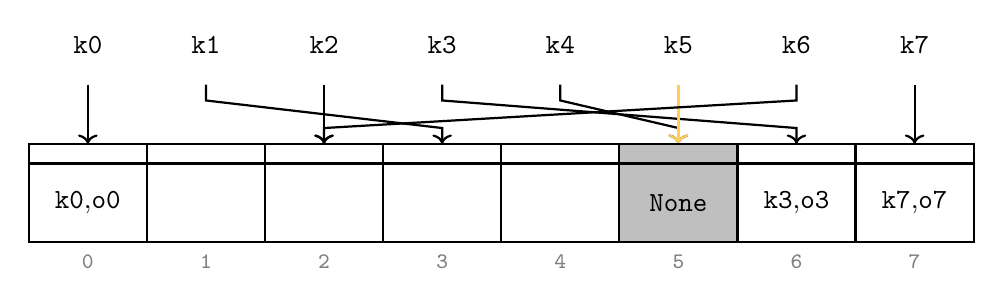
\begin{tikzpicture}

			\begin{scope}
				\begin{scope}[shift={{(-1.5,2)}}]
					\node at (0,0) {\texttt{k0}};
				\end{scope}
				\begin{scope}[shift={{(0,2)}}]
					\node at (0,0) {\texttt{k1}};
				\end{scope}
				\begin{scope}[shift={{(1.5,2)}}]
					\node at (0,0) {\texttt{k2}};
				\end{scope}
				\begin{scope}[shift={{(3,2)}}]
					\node at (0,0) {\texttt{k3}};
				\end{scope}
				\begin{scope}[shift={{(4.5,2)}}]
					\node at (0,0) {\texttt{k4}};
				\end{scope}
				\begin{scope}[shift={{(6,2)}}]
					\node at (0,0) {\texttt{k5}};
				\end{scope}
				\begin{scope}[shift={{(7.5,2)}}]
					\node at (0,0) {\texttt{k6}};
				\end{scope}
				\begin{scope}[shift={{(9,2)}}]
					\node at (0,0) {\texttt{k7}};
				\end{scope}
			\end{scope}

			\begin{scope}
				\tikzset{
					downhead/.style={
							thick,
							postaction={decorate,decoration={markings,mark=at position 1 with {\arrow{>}}}}
						}
				}

				\draw[downhead] (-1.5,1.5) -- ++(0,-0.2) -- (-1.5,0.95) -- ++(0,-0.2);
				\draw[downhead] (0,1.5) -- ++(0,-0.2) -- (3,0.95) -- ++(0,-0.2);
				\draw[downhead] (1.5,1.5) -- ++(0,-0.2) -- (1.5,0.95) -- ++(0,-0.2);
				\draw[downhead] (3,1.5) -- ++(0,-0.2) -- (7.5,0.95) -- ++(0,-0.2);
				\draw[downhead] (4.5,1.5) -- ++(0,-0.2) -- (6,0.95) -- ++(0,-0.2);
				\draw[downhead, myyellow] (6,1.5) -- ++(0,-0.2) -- (6,0.95) -- ++(0,-0.2);
				\draw[downhead] (7.5,1.5) -- ++(0,-0.2) -- (1.5,0.95) -- ++(0,-0.2);
				\draw[downhead] (9,1.5) -- ++(0,-0.2) -- (9,0.95) -- ++(0,-0.2);

			\end{scope}

			\begin{scope}


				\coordinate (mA) at (-1.5,0);
				\coordinate (mB) at (0,0);
				\coordinate (mC) at (1.5,0);
				\coordinate (mD) at (3,0);
				\coordinate (mE) at (4.5,0);
				\coordinate (mF) at (6,0);
				\coordinate (mG) at (7.5,0);
				\coordinate (mH) at (9,0);

				\pic at (mA) {dictnode={white}};
				\pic at (mB) {dictnode={white}};
				\pic at (mC) {dictnode={white}};
				\pic at (mD) {dictnode={white}};
				\pic at (mE) {dictnode={white}};
				\pic at (mF) {dictnode={lightgray}};
				\pic at (mG) {dictnode={white}};
				\pic at (mH) {dictnode={white}};

				\node[smallgraytext] (l1) at (-1.5,-0.75) {\texttt{0}};
				\node[smallgraytext] (l2) at (0,-0.75) {\texttt{1}};
				\node[smallgraytext] (l3) at (1.5,-0.75) {\texttt{2}};
				\node[smallgraytext] (l4) at (3,-0.75) {\texttt{3}};
				\node[smallgraytext] (l5) at (4.5, -0.75) {\texttt{4}};
				\node[smallgraytext] (l6) at (6,-0.75) {\texttt{5}};
				\node[smallgraytext] (l7) at (7.5,-0.75) {\texttt{6}};
				\node[smallgraytext] (l8) at (9,-0.75) {\texttt{7}};

			\end{scope}

			\node at (mA) {\texttt{k0},\texttt{o0}};
			\node at (mG) {\texttt{k3},\texttt{o3}};
			\node at (mH) {\texttt{k7},\texttt{o7}};
			\node at (mF) {\texttt{None}};

		\end{tikzpicture}
	\end{figure}

	\begin{center}
		\footnotesize\color{gray} delete the index specified by the hash value
	\end{center}
\end{frame}

\begin{frame}[fragile]
	\begin{proofbox}
		\begin{lstlisting}[style=mypython]
def delete(self: Dict, key: Key) -> Optional[DictNode]:
    idx = self._hash_fnc(key)
    node = self.buckets[idx].get(0)
    if node is None or node.key is not key:
        return None
    self.buckets[idx] = List()
    self.size -= 1
    return node
\end{lstlisting}
	\end{proofbox}
\end{frame}


\begin{frame}
	A good hash function will be:
	\begin{itemize}
		\item \highlight{\textbf{deterministic}}: \\
		      \footnotesize\color{gray} the same input always produces the same hash value. \normalsize\color{black}
		\item \highlight{\textbf{uniform}}: \\
		      \footnotesize\color{gray} hash values are evenly distributed across the output range, minimizing collisions. \normalsize\color{black}
		\item \highlight{\textbf{efficient}}: \\
		      \footnotesize\color{gray} the hash value should be quick to compute. \normalsize\color{black}
		\item \highlight{\textbf{collision resistant}}: \\
		      \footnotesize\color{gray} rarely maps different inputs to the same hash value. \normalsize\color{black}
		\item \highlight{\textbf{input sensitive}}: \\
		      \footnotesize\color{gray} produces large, unpredictable changes in output when the input changes slightly. \normalsize\color{black}
		\item \highlight{\textbf{bounded}}: \\
		      \footnotesize\color{gray} hash values are bounded between 0 and some positive whole number. \normalsize\color{black}
	\end{itemize}
\end{frame}

\begin{frame}[fragile]
	\vspace{2mm}
	Consider the following hash function:
	\begin{thmbox}
		\begin{lstlisting}[style=mypython]
def simple_hash_fnc(str: String) -> Integer:
    idx = 0
    for chr in str:
        idx += ord(chr) 
    return idx
\end{lstlisting}
	\end{thmbox}
	\begin{center}
		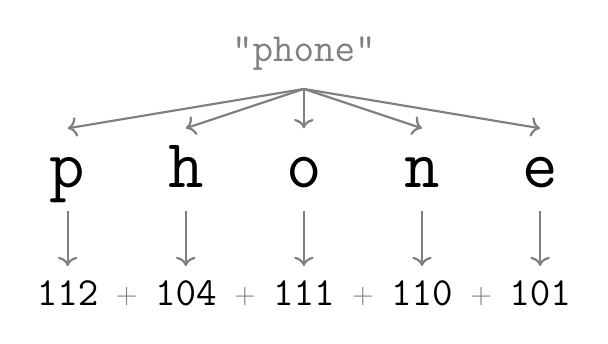
\begin{tikzpicture}
			\node at (0,0.2) {\Large \color{black!50} \texttt{"phone"}};
			\node[anchor=base] at (-3,-1.5) {\Huge\texttt{p}};
			\node[anchor=base] at (-1.5,-1.5) {\Huge\texttt{h}};
			\node[anchor=base] at (0,-1.5) {\Huge\texttt{o}};
			\node[anchor=base] at (1.5,-1.5) {\Huge\texttt{n}};
			\node[anchor=base] at (3,-1.5) {\Huge\texttt{e}};

			\node[anchor=base] at (-3,-3) {\Large\texttt{112}};
			\node[anchor=base, gray] at (-2.25,-2.98) {\normalsize +};

			\node[anchor=base] at (-1.5,-3) {\Large\texttt{104}};
			\node[anchor=base, gray] at (-0.75,-2.98) {\normalsize +};

			\node[anchor=base] at (0,-3) {\Large\texttt{111}};
			\node[anchor=base, gray] at (0.75,-2.98) {\normalsize +};

			\node[anchor=base] at (1.5,-3) {\Large\texttt{110}};
			\node[anchor=base, gray] at (2.25,-2.98) {\normalsize +};

			\node[anchor=base] at (3,-3) {\Large\texttt{101}};

			\draw[->, thick, gray] (0,-0.25) -- (-3,-0.75);
			\draw[->, thick, gray] (0,-0.25) -- (-1.5,-0.75);
			\draw[->, thick, gray] (0,-0.25) -- (0,-0.75);
			\draw[->, thick, gray] (0,-0.25) -- (1.5,-0.75);
			\draw[->, thick, gray] (0,-0.25) -- (3,-0.75);

			\draw[->, thick, gray] (-3,-1.8) -- (-3,-2.5);
			\draw[->, thick, gray] (-1.5,-1.8) -- (-1.5,-2.5);
			\draw[->, thick, gray] (0,-1.8) -- (0,-2.5);
			\draw[->, thick, gray] (1.5,-1.8) -- (1.5,-2.5);
			\draw[->, thick, gray] (3,-1.8) -- (3,-2.5);

		\end{tikzpicture}
	\end{center}
	\begin{center}
		\graytext{the hash value is the sum of the ASCII code for each character}
	\end{center}
\end{frame}

\begin{frame}[fragile]
	Consider the following hash function:
	\begin{thmbox}
		\begin{lstlisting}[style=mypython]
def alternate_hash_fnc(str: String) -> Integer:
    idx = 5381
    for chr in str:
        # hash * 33 + ASCII
        idx = ((idx << 5) + idx) + ord(chr) 
    return idx
\end{lstlisting}
	\end{thmbox}
\end{frame}

\begin{frame}
	Most hash functions are not collision free.

	\begin{figure}
		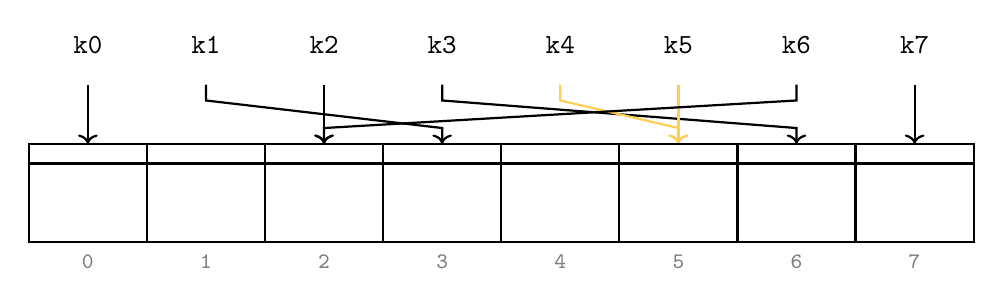
\begin{tikzpicture}

			\begin{scope}
				\begin{scope}[shift={{(-1.5,2)}}]
					\node at (0,0) {\texttt{k0}};
				\end{scope}
				\begin{scope}[shift={{(0,2)}}]
					\node at (0,0) {\texttt{k1}};
				\end{scope}
				\begin{scope}[shift={{(1.5,2)}}]
					\node at (0,0) {\texttt{k2}};
				\end{scope}
				\begin{scope}[shift={{(3,2)}}]
					\node at (0,0) {\texttt{k3}};
				\end{scope}
				\begin{scope}[shift={{(4.5,2)}}]
					\node at (0,0) {\texttt{k4}};
				\end{scope}
				\begin{scope}[shift={{(6,2)}}]
					\node at (0,0) {\texttt{k5}};
				\end{scope}
				\begin{scope}[shift={{(7.5,2)}}]
					\node at (0,0) {\texttt{k6}};
				\end{scope}
				\begin{scope}[shift={{(9,2)}}]
					\node at (0,0) {\texttt{k7}};
				\end{scope}
			\end{scope}

			\begin{scope}
				\tikzset{
					downhead/.style={
							thick,
							postaction={decorate,decoration={markings,mark=at position 1 with {\arrow{>}}}}
						}
				}

				\draw[downhead] (-1.5,1.5) -- ++(0,-0.2) -- (-1.5,0.95) -- ++(0,-0.2);
				\draw[downhead] (0,1.5) -- ++(0,-0.2) -- (3,0.95) -- ++(0,-0.2);
				\draw[downhead] (1.5,1.5) -- ++(0,-0.2) -- (1.5,0.95) -- ++(0,-0.2);
				\draw[downhead] (3,1.5) -- ++(0,-0.2) -- (7.5,0.95) -- ++(0,-0.2);
				\draw[downhead, myyellow] (4.5,1.5) -- ++(0,-0.2) -- (6,0.95) -- ++(0,-0.2);
				\draw[downhead, myyellow] (6,1.5) -- ++(0,-0.2) -- (6,0.95) -- ++(0,-0.2);
				\draw[downhead] (7.5,1.5) -- ++(0,-0.2) -- (1.5,0.95) -- ++(0,-0.2);
				\draw[downhead] (9,1.5) -- ++(0,-0.2) -- (9,0.95) -- ++(0,-0.2);

			\end{scope}

			\begin{scope}


				\coordinate (mA) at (-1.5,0);
				\coordinate (mB) at (0,0);
				\coordinate (mC) at (1.5,0);
				\coordinate (mD) at (3,0);
				\coordinate (mE) at (4.5,0);
				\coordinate (mF) at (6,0);
				\coordinate (mG) at (7.5,0);
				\coordinate (mH) at (9,0);

				\pic at (mA) {dictnode={white}};
				\pic at (mB) {dictnode={white}};
				\pic at (mC) {dictnode={white}};
				\pic at (mD) {dictnode={white}};
				\pic at (mE) {dictnode={white}};
				\pic at (mF) {dictnode={white}};
				\pic at (mG) {dictnode={white}};
				\pic at (mH) {dictnode={white}};

				\node[smallgraytext] (l1) at (-1.5,-0.75) {\texttt{0}};
				\node[smallgraytext] (l2) at (0,-0.75) {\texttt{1}};
				\node[smallgraytext] (l3) at (1.5,-0.75) {\texttt{2}};
				\node[smallgraytext] (l4) at (3,-0.75) {\texttt{3}};
				\node[smallgraytext] (l5) at (4.5, -0.75) {\texttt{4}};
				\node[smallgraytext] (l6) at (6,-0.75) {\texttt{5}};
				\node[smallgraytext] (l7) at (7.5,-0.75) {\texttt{6}};
				\node[smallgraytext] (l8) at (9,-0.75) {\texttt{7}};

			\end{scope}

		\end{tikzpicture}
	\end{figure}

	\begin{center}
		\graytext{\texttt{k4} and \texttt{k5} both hash to the same index (5)}
	\end{center}
\end{frame}

\begin{frame}
	Collisions can be resolved in two main ways:
	\begin{itemize}
		\item \highlight{\textbf{open addressing (probing)}}: \\ \footnotesize\color{gray} whenever a collision occurs, find another empty slot; keys are stored with their values since different keys may hash to the same slot. \normalsize\color{black}
		\item \highlight{\textbf{closed addressing (chaining)}}: \\
		      \footnotesize\color{gray}
		      whenever a collision occurs, use a list to store multiple nodes; keys are stored with their nodes since different keys will map to the same slot.
		      \normalsize\color{black}
	\end{itemize}
\end{frame}

\begin{frame}[fragile]
	To use \textit{open addressing (probing)}, we make use of the \texttt{probe\_fnc} attribute in \texttt{Dict} class:
	\begin{itemize}
		\item \highlight{\textbf{linear probing}}: \\
		      \footnotesize\color{gray} on a collision, move linearly many step each time ($1, 2, 3, \dots$) \\
		      simple but can lead to clustering \normalsize\color{black}
		      \begin{lstlisting}[style=mypython]
def probe_fnc(self: Dict, step: Integer) -> Integer:
    return step
\end{lstlisting}

		\item \highlight{\textbf{quadratic probing}}: \\
		      \footnotesize\color{gray} on a collision, move quadratically many steps each time ($1^2$, $2^2$, $3^2$, $\dots$) \\
		      reduces clustering but may not visit all slots \normalsize\color{black}
		      \begin{lstlisting}[style=mypython]
def probe_fnc(self: Dict, step: Integer) -> Integer:
    return step * step
\end{lstlisting}
	\end{itemize}
\end{frame}

\begin{frame}
	\begin{center}
		\highlight{\textbf{insert}} \\[1mm]
		\footnotesize\color{gray} \texttt{insert(k4, o4)} with linear probing
	\end{center}

	\begin{figure}
		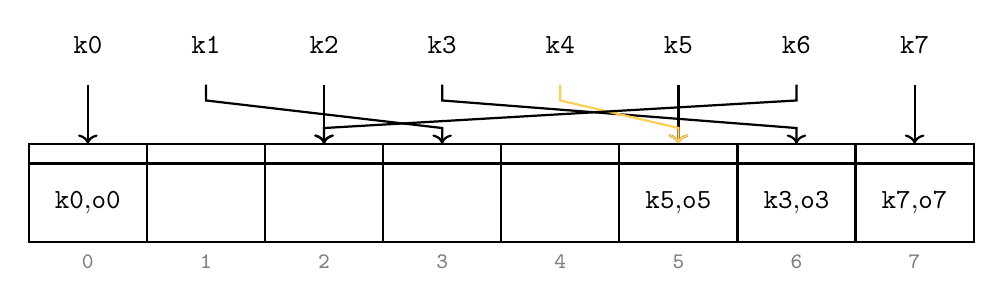
\begin{tikzpicture}

			\begin{scope}
				\begin{scope}[shift={{(-1.5,2)}}]
					\node at (0,0) {\texttt{k0}};
				\end{scope}
				\begin{scope}[shift={{(0,2)}}]
					\node at (0,0) {\texttt{k1}};
				\end{scope}
				\begin{scope}[shift={{(1.5,2)}}]
					\node at (0,0) {\texttt{k2}};
				\end{scope}
				\begin{scope}[shift={{(3,2)}}]
					\node at (0,0) {\texttt{k3}};
				\end{scope}
				\begin{scope}[shift={{(4.5,2)}}]
					\node at (0,0) {\texttt{k4}};
				\end{scope}
				\begin{scope}[shift={{(6,2)}}]
					\node at (0,0) {\texttt{k5}};
				\end{scope}
				\begin{scope}[shift={{(7.5,2)}}]
					\node at (0,0) {\texttt{k6}};
				\end{scope}
				\begin{scope}[shift={{(9,2)}}]
					\node at (0,0) {\texttt{k7}};
				\end{scope}
			\end{scope}

			\begin{scope}
				\tikzset{
					downhead/.style={
							thick,
							postaction={decorate,decoration={markings,mark=at position 1 with {\arrow{>}}}}
						}
				}

				\draw[downhead] (-1.5,1.5) -- ++(0,-0.2) -- (-1.5,0.95) -- ++(0,-0.2);
				\draw[downhead] (0,1.5) -- ++(0,-0.2) -- (3,0.95) -- ++(0,-0.2);
				\draw[downhead] (1.5,1.5) -- ++(0,-0.2) -- (1.5,0.95) -- ++(0,-0.2);
				\draw[downhead] (3,1.5) -- ++(0,-0.2) -- (7.5,0.95) -- ++(0,-0.2);
				\draw[downhead] (6,1.5) -- ++(0,-0.2) -- (6,0.95) -- ++(0,-0.2);
				\draw[downhead, myyellow] (4.5,1.5) -- ++(0,-0.2) -- (6,0.95) -- ++(0,-0.2);
				\draw[downhead] (7.5,1.5) -- ++(0,-0.2) -- (1.5,0.95) -- ++(0,-0.2);
				\draw[downhead] (9,1.5) -- ++(0,-0.2) -- (9,0.95) -- ++(0,-0.2);

			\end{scope}

			\begin{scope}


				\coordinate (mA) at (-1.5,0);
				\coordinate (mB) at (0,0);
				\coordinate (mC) at (1.5,0);
				\coordinate (mD) at (3,0);
				\coordinate (mE) at (4.5,0);
				\coordinate (mF) at (6,0);
				\coordinate (mG) at (7.5,0);
				\coordinate (mH) at (9,0);

				\pic at (mA) {dictnode={white}};
				\pic at (mB) {dictnode={white}};
				\pic at (mC) {dictnode={white}};
				\pic at (mD) {dictnode={white}};
				\pic at (mE) {dictnode={white}};
				\pic at (mF) {dictnode={white}};
				\pic at (mG) {dictnode={white}};
				\pic at (mH) {dictnode={white}};

				\node[smallgraytext] (l1) at (-1.5,-0.75) {\texttt{0}};
				\node[smallgraytext] (l2) at (0,-0.75) {\texttt{1}};
				\node[smallgraytext] (l3) at (1.5,-0.75) {\texttt{2}};
				\node[smallgraytext] (l4) at (3,-0.75) {\texttt{3}};
				\node[smallgraytext] (l5) at (4.5, -0.75) {\texttt{4}};
				\node[smallgraytext] (l6) at (6,-0.75) {\texttt{5}};
				\node[smallgraytext] (l7) at (7.5,-0.75) {\texttt{6}};
				\node[smallgraytext] (l8) at (9,-0.75) {\texttt{7}};

			\end{scope}

			\node at (mA) {\texttt{k0},\texttt{o0}};
			\node at (mG) {\texttt{k3},\texttt{o3}};
			\node at (mH) {\texttt{k7},\texttt{o7}};
			\node at (mF) {\texttt{k5},\texttt{o5}};

		\end{tikzpicture}
	\end{figure}

	\begin{center}
		\footnotesize\color{gray} compute the hash value of the key
	\end{center}
\end{frame}

\begin{frame}
	\begin{center}
		\highlight{\textbf{insert}} \\[1mm]
		\footnotesize\color{gray} \texttt{insert(k4, o4)} with linear probing
	\end{center}

	\begin{figure}
		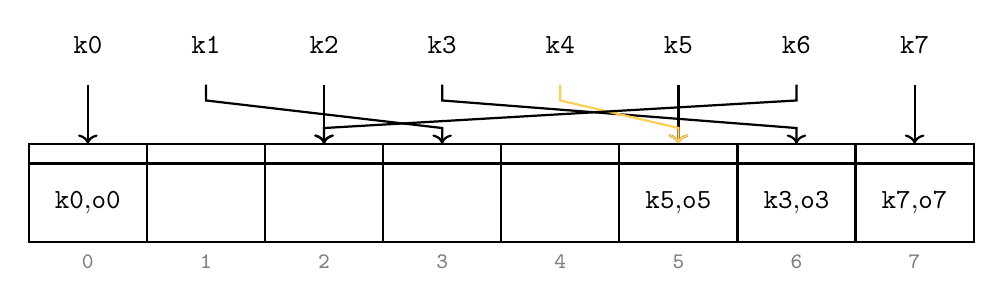
\begin{tikzpicture}

			\begin{scope}
				\begin{scope}[shift={{(-1.5,2)}}]
					\node at (0,0) {\texttt{k0}};
				\end{scope}
				\begin{scope}[shift={{(0,2)}}]
					\node at (0,0) {\texttt{k1}};
				\end{scope}
				\begin{scope}[shift={{(1.5,2)}}]
					\node at (0,0) {\texttt{k2}};
				\end{scope}
				\begin{scope}[shift={{(3,2)}}]
					\node at (0,0) {\texttt{k3}};
				\end{scope}
				\begin{scope}[shift={{(4.5,2)}}]
					\node at (0,0) {\texttt{k4}};
				\end{scope}
				\begin{scope}[shift={{(6,2)}}]
					\node at (0,0) {\texttt{k5}};
				\end{scope}
				\begin{scope}[shift={{(7.5,2)}}]
					\node at (0,0) {\texttt{k6}};
				\end{scope}
				\begin{scope}[shift={{(9,2)}}]
					\node at (0,0) {\texttt{k7}};
				\end{scope}
			\end{scope}

			\begin{scope}
				\tikzset{
					downhead/.style={
							thick,
							postaction={decorate,decoration={markings,mark=at position 1 with {\arrow{>}}}}
						}
				}

				\draw[downhead] (-1.5,1.5) -- ++(0,-0.2) -- (-1.5,0.95) -- ++(0,-0.2);
				\draw[downhead] (0,1.5) -- ++(0,-0.2) -- (3,0.95) -- ++(0,-0.2);
				\draw[downhead] (1.5,1.5) -- ++(0,-0.2) -- (1.5,0.95) -- ++(0,-0.2);
				\draw[downhead] (3,1.5) -- ++(0,-0.2) -- (7.5,0.95) -- ++(0,-0.2);
				\draw[downhead] (6,1.5) -- ++(0,-0.2) -- (6,0.95) -- ++(0,-0.2);
				\draw[downhead, myyellow] (4.5,1.5) -- ++(0,-0.2) -- (6,0.95) -- ++(0,-0.2);
				\draw[downhead] (7.5,1.5) -- ++(0,-0.2) -- (1.5,0.95) -- ++(0,-0.2);
				\draw[downhead] (9,1.5) -- ++(0,-0.2) -- (9,0.95) -- ++(0,-0.2);

			\end{scope}

			\begin{scope}


				\coordinate (mA) at (-1.5,0);
				\coordinate (mB) at (0,0);
				\coordinate (mC) at (1.5,0);
				\coordinate (mD) at (3,0);
				\coordinate (mE) at (4.5,0);
				\coordinate (mF) at (6,0);
				\coordinate (mG) at (7.5,0);
				\coordinate (mH) at (9,0);

				\pic at (mA) {dictnode={white}};
				\pic at (mB) {dictnode={white}};
				\pic at (mC) {dictnode={white}};
				\pic at (mD) {dictnode={white}};
				\pic at (mE) {dictnode={white}};
				\pic at (mF) {dictnode={white}};
				\pic at (mG) {dictnode={white}};
				\pic at (mH) {dictnode={white}};

				\node[smallgraytext] (l1) at (-1.5,-0.75) {\texttt{0}};
				\node[smallgraytext] (l2) at (0,-0.75) {\texttt{1}};
				\node[smallgraytext] (l3) at (1.5,-0.75) {\texttt{2}};
				\node[smallgraytext] (l4) at (3,-0.75) {\texttt{3}};
				\node[smallgraytext] (l5) at (4.5, -0.75) {\texttt{4}};
				\node[smallgraytext] (l6) at (6,-0.75) {\texttt{5}};
				\node[smallgraytext] (l7) at (7.5,-0.75) {\texttt{6}};
				\node[smallgraytext] (l8) at (9,-0.75) {\texttt{7}};

			\end{scope}

			\node at (mA) {\texttt{k0},\texttt{o0}};
			\node at (mG) {\texttt{k3},\texttt{o3}};
			\node at (mH) {\texttt{k7},\texttt{o7}};
			\node at (mF) {\texttt{k5},\texttt{o5}};

		\end{tikzpicture}
	\end{figure}

	\begin{center}
		\footnotesize\color{gray} find the next available position (stepping 1, 2, 3, $\dots$)
	\end{center}
\end{frame}

\begin{frame}
	\begin{center}
		\highlight{\textbf{insert}} \\[1mm]
		\footnotesize\color{gray} \texttt{insert(k4, o4)} with quadratic probing
	\end{center}

	\begin{figure}
		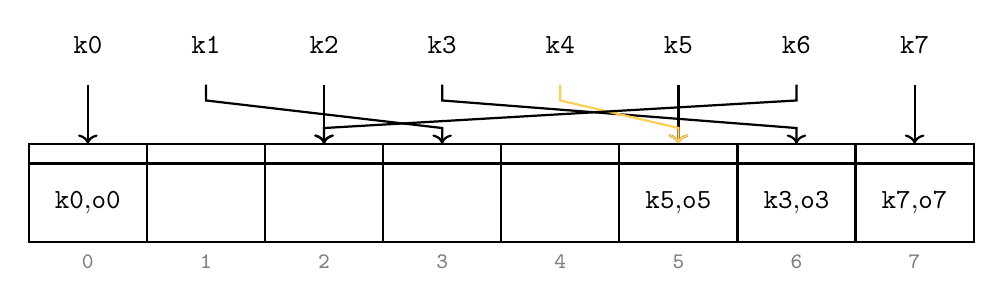
\begin{tikzpicture}

			\begin{scope}
				\begin{scope}[shift={{(-1.5,2)}}]
					\node at (0,0) {\texttt{k0}};
				\end{scope}
				\begin{scope}[shift={{(0,2)}}]
					\node at (0,0) {\texttt{k1}};
				\end{scope}
				\begin{scope}[shift={{(1.5,2)}}]
					\node at (0,0) {\texttt{k2}};
				\end{scope}
				\begin{scope}[shift={{(3,2)}}]
					\node at (0,0) {\texttt{k3}};
				\end{scope}
				\begin{scope}[shift={{(4.5,2)}}]
					\node at (0,0) {\texttt{k4}};
				\end{scope}
				\begin{scope}[shift={{(6,2)}}]
					\node at (0,0) {\texttt{k5}};
				\end{scope}
				\begin{scope}[shift={{(7.5,2)}}]
					\node at (0,0) {\texttt{k6}};
				\end{scope}
				\begin{scope}[shift={{(9,2)}}]
					\node at (0,0) {\texttt{k7}};
				\end{scope}
			\end{scope}

			\begin{scope}
				\tikzset{
					downhead/.style={
							thick,
							postaction={decorate,decoration={markings,mark=at position 1 with {\arrow{>}}}}
						}
				}

				\draw[downhead] (-1.5,1.5) -- ++(0,-0.2) -- (-1.5,0.95) -- ++(0,-0.2);
				\draw[downhead] (0,1.5) -- ++(0,-0.2) -- (3,0.95) -- ++(0,-0.2);
				\draw[downhead] (1.5,1.5) -- ++(0,-0.2) -- (1.5,0.95) -- ++(0,-0.2);
				\draw[downhead] (3,1.5) -- ++(0,-0.2) -- (7.5,0.95) -- ++(0,-0.2);
				\draw[downhead] (6,1.5) -- ++(0,-0.2) -- (6,0.95) -- ++(0,-0.2);
				\draw[downhead, myyellow] (4.5,1.5) -- ++(0,-0.2) -- (6,0.95) -- ++(0,-0.2);
				\draw[downhead] (7.5,1.5) -- ++(0,-0.2) -- (1.5,0.95) -- ++(0,-0.2);
				\draw[downhead] (9,1.5) -- ++(0,-0.2) -- (9,0.95) -- ++(0,-0.2);

			\end{scope}

			\begin{scope}


				\coordinate (mA) at (-1.5,0);
				\coordinate (mB) at (0,0);
				\coordinate (mC) at (1.5,0);
				\coordinate (mD) at (3,0);
				\coordinate (mE) at (4.5,0);
				\coordinate (mF) at (6,0);
				\coordinate (mG) at (7.5,0);
				\coordinate (mH) at (9,0);

				\pic at (mA) {dictnode={white}};
				\pic at (mB) {dictnode={white}};
				\pic at (mC) {dictnode={white}};
				\pic at (mD) {dictnode={white}};
				\pic at (mE) {dictnode={white}};
				\pic at (mF) {dictnode={white}};
				\pic at (mG) {dictnode={white}};
				\pic at (mH) {dictnode={white}};

				\node[smallgraytext] (l1) at (-1.5,-0.75) {\texttt{0}};
				\node[smallgraytext] (l2) at (0,-0.75) {\texttt{1}};
				\node[smallgraytext] (l3) at (1.5,-0.75) {\texttt{2}};
				\node[smallgraytext] (l4) at (3,-0.75) {\texttt{3}};
				\node[smallgraytext] (l5) at (4.5, -0.75) {\texttt{4}};
				\node[smallgraytext] (l6) at (6,-0.75) {\texttt{5}};
				\node[smallgraytext] (l7) at (7.5,-0.75) {\texttt{6}};
				\node[smallgraytext] (l8) at (9,-0.75) {\texttt{7}};

			\end{scope}

			\node at (mA) {\texttt{k0},\texttt{o0}};
			\node at (mG) {\texttt{k3},\texttt{o3}};
			\node at (mH) {\texttt{k7},\texttt{o7}};
			\node at (mF) {\texttt{k5},\texttt{o5}};

		\end{tikzpicture}
	\end{figure}

	\begin{center}
		\footnotesize\color{gray} compute the hash value of the key
	\end{center}
\end{frame}

\begin{frame}
	\begin{center}
		\highlight{\textbf{insert}} \\[1mm]
		\footnotesize\color{gray} \texttt{insert(k4, o4)} with quadratic probing
	\end{center}


	\begin{figure}
		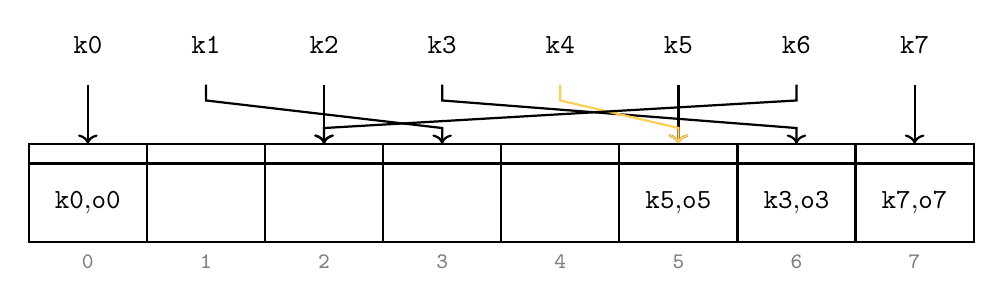
\begin{tikzpicture}

			\begin{scope}
				\begin{scope}[shift={{(-1.5,2)}}]
					\node at (0,0) {\texttt{k0}};
				\end{scope}
				\begin{scope}[shift={{(0,2)}}]
					\node at (0,0) {\texttt{k1}};
				\end{scope}
				\begin{scope}[shift={{(1.5,2)}}]
					\node at (0,0) {\texttt{k2}};
				\end{scope}
				\begin{scope}[shift={{(3,2)}}]
					\node at (0,0) {\texttt{k3}};
				\end{scope}
				\begin{scope}[shift={{(4.5,2)}}]
					\node at (0,0) {\texttt{k4}};
				\end{scope}
				\begin{scope}[shift={{(6,2)}}]
					\node at (0,0) {\texttt{k5}};
				\end{scope}
				\begin{scope}[shift={{(7.5,2)}}]
					\node at (0,0) {\texttt{k6}};
				\end{scope}
				\begin{scope}[shift={{(9,2)}}]
					\node at (0,0) {\texttt{k7}};
				\end{scope}
			\end{scope}

			\begin{scope}
				\tikzset{
					downhead/.style={
							thick,
							postaction={decorate,decoration={markings,mark=at position 1 with {\arrow{>}}}}
						}
				}

				\draw[downhead] (-1.5,1.5) -- ++(0,-0.2) -- (-1.5,0.95) -- ++(0,-0.2);
				\draw[downhead] (0,1.5) -- ++(0,-0.2) -- (3,0.95) -- ++(0,-0.2);
				\draw[downhead] (1.5,1.5) -- ++(0,-0.2) -- (1.5,0.95) -- ++(0,-0.2);
				\draw[downhead] (3,1.5) -- ++(0,-0.2) -- (7.5,0.95) -- ++(0,-0.2);
				\draw[downhead] (6,1.5) -- ++(0,-0.2) -- (6,0.95) -- ++(0,-0.2);
				\draw[downhead, myyellow] (4.5,1.5) -- ++(0,-0.2) -- (6,0.95) -- ++(0,-0.2);
				\draw[downhead] (7.5,1.5) -- ++(0,-0.2) -- (1.5,0.95) -- ++(0,-0.2);
				\draw[downhead] (9,1.5) -- ++(0,-0.2) -- (9,0.95) -- ++(0,-0.2);

			\end{scope}

			\begin{scope}


				\coordinate (mA) at (-1.5,0);
				\coordinate (mB) at (0,0);
				\coordinate (mC) at (1.5,0);
				\coordinate (mD) at (3,0);
				\coordinate (mE) at (4.5,0);
				\coordinate (mF) at (6,0);
				\coordinate (mG) at (7.5,0);
				\coordinate (mH) at (9,0);

				\pic at (mA) {dictnode={white}};
				\pic at (mB) {dictnode={white}};
				\pic at (mC) {dictnode={white}};
				\pic at (mD) {dictnode={white}};
				\pic at (mE) {dictnode={white}};
				\pic at (mF) {dictnode={white}};
				\pic at (mG) {dictnode={white}};
				\pic at (mH) {dictnode={white}};

				\node[smallgraytext] (l1) at (-1.5,-0.75) {\texttt{0}};
				\node[smallgraytext] (l2) at (0,-0.75) {\texttt{1}};
				\node[smallgraytext] (l3) at (1.5,-0.75) {\texttt{2}};
				\node[smallgraytext] (l4) at (3,-0.75) {\texttt{3}};
				\node[smallgraytext] (l5) at (4.5, -0.75) {\texttt{4}};
				\node[smallgraytext] (l6) at (6,-0.75) {\texttt{5}};
				\node[smallgraytext] (l7) at (7.5,-0.75) {\texttt{6}};
				\node[smallgraytext] (l8) at (9,-0.75) {\texttt{7}};

			\end{scope}

			\node at (mA) {\texttt{k0},\texttt{o0}};
			\node at (mG) {\texttt{k3},\texttt{o3}};
			\node at (mH) {\texttt{k7},\texttt{o7}};
			\node at (mF) {\texttt{k5},\texttt{o5}};

		\end{tikzpicture}
	\end{figure}

	\begin{center}
		\footnotesize\color{gray} find the next available position (stepping 1, 4, 9, $\dots$)
	\end{center}
\end{frame}

\begin{frame}[fragile]
	\begin{proofbox}
		\begin{lstlisting}[style=mypython]
def get(self: Dict, key: Key) -> Optional[DictNode]:
    start = self._hash_fnc(key)
    idx = start
    step = 0
    
    while self.buckets[idx] is not None:
        node = self.buckets[idx]
        if node.key is key:
            return node
        step += 1
        idx = start + self.probe_fnc(step)
        if idx >= start:
            break
    return None
\end{lstlisting}
	\end{proofbox}
\end{frame}

\begin{frame}[fragile]
	\begin{proofbox}
		\begin{lstlisting}[style=mypython]
def insert(self: Dict, key: Key, obj: Object) -> Optional[DictNode]:
    if self.size >= self.capacity:
        self._resize()
    idx = self._hash_fnc(key)
    step = 0
    while self.buckets[idx] is not None, Del:
        node = self.buckets[idx]
        if node(0) == key:
            self.buckets[idx] = DictNode(key, obj)
            return self.buckets[idx]
        step += 1
        idx = start + self.probe_fnc(step)
        if idx >= start: # assume full
            self._resize()
            return self.insert(key, obj)
    self.buckets[idx] = DictNode(key, obj)
    self.size += 1
    return self.buckets[idx]
\end{lstlisting}
	\end{proofbox}
\end{frame}

\begin{frame}[fragile]
	\begin{proofbox}
		\begin{lstlisting}[style=mypython]
def delete(self: Dict, key: Key) -> Optional[DictNode]:
    start = self._hash_fnc(key)
    idx = start
    step = 0
    
    while self.buckets[idx] is not None:
        node = self.buckets[idx]
        if node.key is key:
            self.buckets[idx] = None
            self.count -= 1
            return node
        step += 1
        idx = start + self.probe_fnc(step)
        if idx >= start:
            break
    return None
\end{lstlisting}
	\end{proofbox}
\end{frame}

\begin{frame}[fragile]
	To use \textit{closed addressing (chaining}), we make use of the \texttt{next} attribute within the \texttt{DictNode} class.
\end{frame}


\begin{frame}
	\begin{center}
		\highlight{\textbf{insert}} \\[1mm]
		\footnotesize\color{gray} \texttt{insert(k4, o4)} with chaining
	\end{center}


	\begin{figure}
		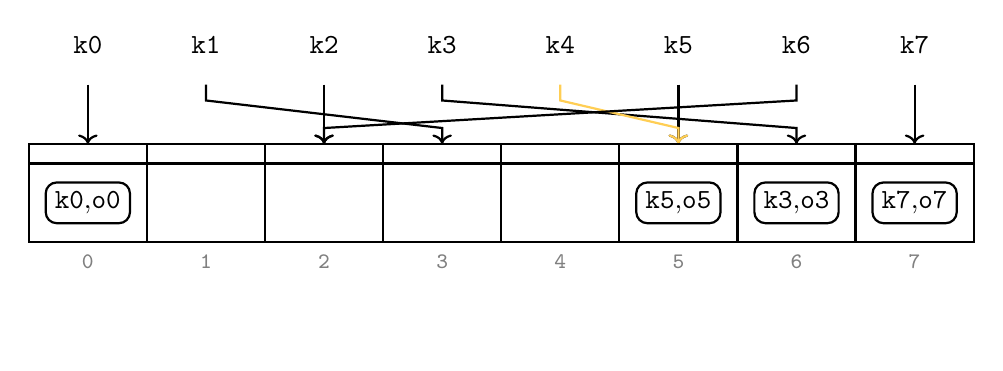
\begin{tikzpicture}

			\begin{scope}
				\begin{scope}[shift={{(-1.5,2)}}]
					\node at (0,0) {\texttt{k0}};
				\end{scope}
				\begin{scope}[shift={{(0,2)}}]
					\node at (0,0) {\texttt{k1}};
				\end{scope}
				\begin{scope}[shift={{(1.5,2)}}]
					\node at (0,0) {\texttt{k2}};
				\end{scope}
				\begin{scope}[shift={{(3,2)}}]
					\node at (0,0) {\texttt{k3}};
				\end{scope}
				\begin{scope}[shift={{(4.5,2)}}]
					\node at (0,0) {\texttt{k4}};
				\end{scope}
				\begin{scope}[shift={{(6,2)}}]
					\node at (0,0) {\texttt{k5}};
				\end{scope}
				\begin{scope}[shift={{(7.5,2)}}]
					\node at (0,0) {\texttt{k6}};
				\end{scope}
				\begin{scope}[shift={{(9,2)}}]
					\node at (0,0) {\texttt{k7}};
				\end{scope}
			\end{scope}

			\begin{scope}
				\tikzset{
					downhead/.style={
							thick,
							postaction={decorate,decoration={markings,mark=at position 1 with {\arrow{>}}}}
						}
				}

				\draw[downhead] (-1.5,1.5) -- ++(0,-0.2) -- (-1.5,0.95) -- ++(0,-0.2);
				\draw[downhead] (0,1.5) -- ++(0,-0.2) -- (3,0.95) -- ++(0,-0.2);
				\draw[downhead] (1.5,1.5) -- ++(0,-0.2) -- (1.5,0.95) -- ++(0,-0.2);
				\draw[downhead] (3,1.5) -- ++(0,-0.2) -- (7.5,0.95) -- ++(0,-0.2);
				\draw[downhead] (6,1.5) -- ++(0,-0.2) -- (6,0.95) -- ++(0,-0.2);
				\draw[downhead, myyellow] (4.5,1.5) -- ++(0,-0.2) -- (6,0.95) -- ++(0,-0.2);
				\draw[downhead] (7.5,1.5) -- ++(0,-0.2) -- (1.5,0.95) -- ++(0,-0.2);
				\draw[downhead] (9,1.5) -- ++(0,-0.2) -- (9,0.95) -- ++(0,-0.2);

			\end{scope}

			\begin{scope}


				\coordinate (mA) at (-1.5,0);
				\coordinate (mB) at (0,0);
				\coordinate (mC) at (1.5,0);
				\coordinate (mD) at (3,0);
				\coordinate (mE) at (4.5,0);
				\coordinate (mF) at (6,0);
				\coordinate (mG) at (7.5,0);
				\coordinate (mH) at (9,0);

				\pic at (mA) {dictnode={white}};
				\pic at (mB) {dictnode={white}};
				\pic at (mC) {dictnode={white}};
				\pic at (mD) {dictnode={white}};
				\pic at (mE) {dictnode={white}};
				\pic at (mF) {dictnode={white}};
				\pic at (mG) {dictnode={white}};
				\pic at (mH) {dictnode={white}};

				\node[smallgraytext] (l1) at (-1.5,-0.75) {\texttt{0}};
				\node[smallgraytext] (l2) at (0,-0.75) {\texttt{1}};
				\node[smallgraytext] (l3) at (1.5,-0.75) {\texttt{2}};
				\node[smallgraytext] (l4) at (3,-0.75) {\texttt{3}};
				\node[smallgraytext] (l5) at (4.5, -0.75) {\texttt{4}};
				\node[smallgraytext] (l6) at (6,-0.75) {\texttt{5}};
				\node[smallgraytext] (l7) at (7.5,-0.75) {\texttt{6}};
				\node[smallgraytext] (l8) at (9,-0.75) {\texttt{7}};

			\end{scope}

			\node[draw=black, thick, rounded corners, rectangle] at (mA) {\texttt{k0},\texttt{o0}};
			\node[draw=black, thick, rounded corners, rectangle] at (mG) {\texttt{k3},\texttt{o3}};
			\node[draw=black, thick, rounded corners, rectangle] at (mH) {\texttt{k7},\texttt{o7}};

			\node[draw=black, thick, rounded corners, rectangle] (ll1) at (mF) {\texttt{k5},\texttt{o5}};
			\node[opacity=0, draw=black,thick, rounded corners, rectangle, yshift=-15mm] (ll2) at (mF) {\texttt{k4},\texttt{o4}};
			\draw[->, thick, opacity=0] (ll1) edge[bend left] (ll2);
			\draw[<-, thick, opacity=0] (ll1) edge[bend right] (ll2);

		\end{tikzpicture}
	\end{figure}

	\begin{center}
		\footnotesize\color{gray} compute the hash value of the key
	\end{center}
\end{frame}

\begin{frame}
	\begin{center}
		\highlight{\textbf{insert}} \\[1mm]
		\footnotesize\color{gray} \texttt{insert(k4, o4)} with chaining
	\end{center}

	\begin{figure}
		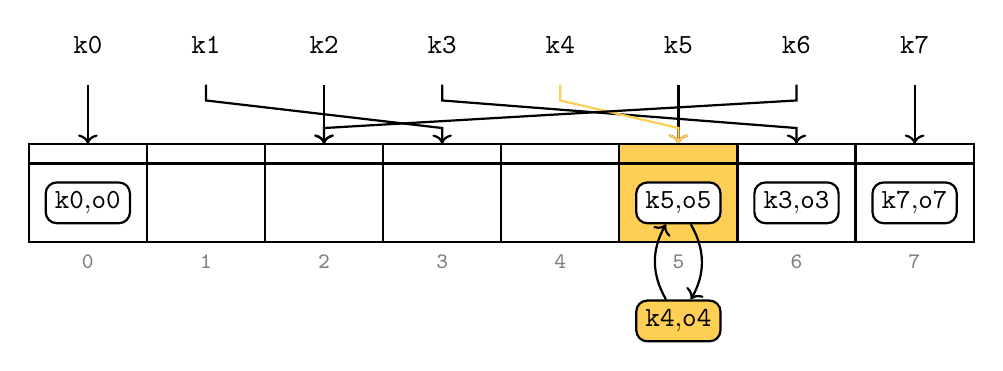
\begin{tikzpicture}

			\begin{scope}
				\begin{scope}[shift={{(-1.5,2)}}]
					\node at (0,0) {\texttt{k0}};
				\end{scope}
				\begin{scope}[shift={{(0,2)}}]
					\node at (0,0) {\texttt{k1}};
				\end{scope}
				\begin{scope}[shift={{(1.5,2)}}]
					\node at (0,0) {\texttt{k2}};
				\end{scope}
				\begin{scope}[shift={{(3,2)}}]
					\node at (0,0) {\texttt{k3}};
				\end{scope}
				\begin{scope}[shift={{(4.5,2)}}]
					\node at (0,0) {\texttt{k4}};
				\end{scope}
				\begin{scope}[shift={{(6,2)}}]
					\node at (0,0) {\texttt{k5}};
				\end{scope}
				\begin{scope}[shift={{(7.5,2)}}]
					\node at (0,0) {\texttt{k6}};
				\end{scope}
				\begin{scope}[shift={{(9,2)}}]
					\node at (0,0) {\texttt{k7}};
				\end{scope}
			\end{scope}

			\begin{scope}
				\tikzset{
					downhead/.style={
							thick,
							postaction={decorate,decoration={markings,mark=at position 1 with {\arrow{>}}}}
						}
				}

				\draw[downhead] (-1.5,1.5) -- ++(0,-0.2) -- (-1.5,0.95) -- ++(0,-0.2);
				\draw[downhead] (0,1.5) -- ++(0,-0.2) -- (3,0.95) -- ++(0,-0.2);
				\draw[downhead] (1.5,1.5) -- ++(0,-0.2) -- (1.5,0.95) -- ++(0,-0.2);
				\draw[downhead] (3,1.5) -- ++(0,-0.2) -- (7.5,0.95) -- ++(0,-0.2);
				\draw[downhead] (6,1.5) -- ++(0,-0.2) -- (6,0.95) -- ++(0,-0.2);
				\draw[downhead, myyellow] (4.5,1.5) -- ++(0,-0.2) -- (6,0.95) -- ++(0,-0.2);
				\draw[downhead] (7.5,1.5) -- ++(0,-0.2) -- (1.5,0.95) -- ++(0,-0.2);
				\draw[downhead] (9,1.5) -- ++(0,-0.2) -- (9,0.95) -- ++(0,-0.2);

			\end{scope}

			\begin{scope}


				\coordinate (mA) at (-1.5,0);
				\coordinate (mB) at (0,0);
				\coordinate (mC) at (1.5,0);
				\coordinate (mD) at (3,0);
				\coordinate (mE) at (4.5,0);
				\coordinate (mF) at (6,0);
				\coordinate (mG) at (7.5,0);
				\coordinate (mH) at (9,0);

				\pic at (mA) {dictnode={white}};
				\pic at (mB) {dictnode={white}};
				\pic at (mC) {dictnode={white}};
				\pic at (mD) {dictnode={white}};
				\pic at (mE) {dictnode={white}};
				\pic at (mF) {dictnode={myyellow}};
				\pic at (mG) {dictnode={white}};
				\pic at (mH) {dictnode={white}};

				\node[smallgraytext] (l1) at (-1.5,-0.75) {\texttt{0}};
				\node[smallgraytext] (l2) at (0,-0.75) {\texttt{1}};
				\node[smallgraytext] (l3) at (1.5,-0.75) {\texttt{2}};
				\node[smallgraytext] (l4) at (3,-0.75) {\texttt{3}};
				\node[smallgraytext] (l5) at (4.5, -0.75) {\texttt{4}};
				\node[smallgraytext] (l6) at (6,-0.75) {\texttt{5}};
				\node[smallgraytext] (l7) at (7.5,-0.75) {\texttt{6}};
				\node[smallgraytext] (l8) at (9,-0.75) {\texttt{7}};

			\end{scope}

			\node[draw=black, thick, rounded corners, rectangle] at (mA) {\texttt{k0},\texttt{o0}};
			\node[draw=black, thick, rounded corners, rectangle] at (mG) {\texttt{k3},\texttt{o3}};
			\node[draw=black, thick, rounded corners, rectangle] at (mH) {\texttt{k7},\texttt{o7}};

			\node[draw=black, thick, fill=white, rounded corners, rectangle] (ll1) at (mF) {\texttt{k5},\texttt{o5}};
			\node[draw=black,thick, fill=myyellow, rounded corners, rectangle, yshift=-15mm] (ll2) at (mF) {\texttt{k4},\texttt{o4}};
			\draw[->, thick] (ll1) edge[bend left] (ll2);
			\draw[<-, thick] (ll1) edge[bend right] (ll2);

		\end{tikzpicture}
	\end{figure}

	\begin{center}
		\footnotesize\color{gray} chain the key-object pair
	\end{center}
\end{frame}

\begin{frame}[fragile]
	\begin{proofbox}
		\begin{lstlisting}[style=mypython]
def get(self: Dict, key: Key) -> Optional[DictNode]:
    idx = self._hash_fnc(key)
    lst = self.buckets[idx]
    return lst.get(key)
\end{lstlisting}
	\end{proofbox}
\end{frame}

\begin{frame}[fragile]
	\begin{proofbox}
		\begin{lstlisting}[style=mypython]
def insert(self: Dict, obj: Object) -> Optional[DictNode]:
    idx = self._hash_fnc(key) 
    lst = self.buckets[self._hash_fnc(key)]
    return lst.insert(key, obj)
\end{lstlisting}
	\end{proofbox}
\end{frame}

\begin{frame}[fragile]
	\begin{proofbox}
		\begin{lstlisting}[style=mypython]
def delete(self: Dict, key: Key) -> Optional[DictNode]:
    idx = self._hash_fnc(key)
    lst = self.buckets[idx]
    return lst.delete(key)
\end{lstlisting}
	\end{proofbox}
\end{frame}

\begin{frame}
	\begin{table}
		\begin{tabular}{@{} r | l @{} }
			\highlight{\textbf{Property}}            &                                              \\[1mm]\hline
			\multirow{1}{*}{Time Complexity}         &                                              \\
			\color{gray}\footnotesize\texttt{insert} & \color{gray}\footnotesize $\hat{O}(\log(N))$ \\[1mm]
			\color{gray}\footnotesize\texttt{get}    & \color{gray}\footnotesize $\hat{O}(\log(N))$ \\[1mm]
			\color{gray}\footnotesize\texttt{delete} & \color{gray}\footnotesize $\hat{O}(\log(N))$ \\[1mm]
			Space Complexity                         & $O(N)$
		\end{tabular}
	\end{table}
	\begin{center}
		\footnotesize\color{gray} properties of the \texttt{Dict} data-structure (via Hash Tables)
	\end{center}
	\renewcommand\thefootnote{}\footnotetext{\color{gray} Assumptions: $N = $ \texttt{Dict.size}}
\end{frame}

\end{document}
